\section{LeNet-5}
LeNet-5 \cite{Lenet5} is the name of a certain architecture of a convolutional network designed for document recognition (handwritten, machine printed characters) developed by Yan Lecun \textit{et al}.\\

\begin{figure}[htb]
  \centering
  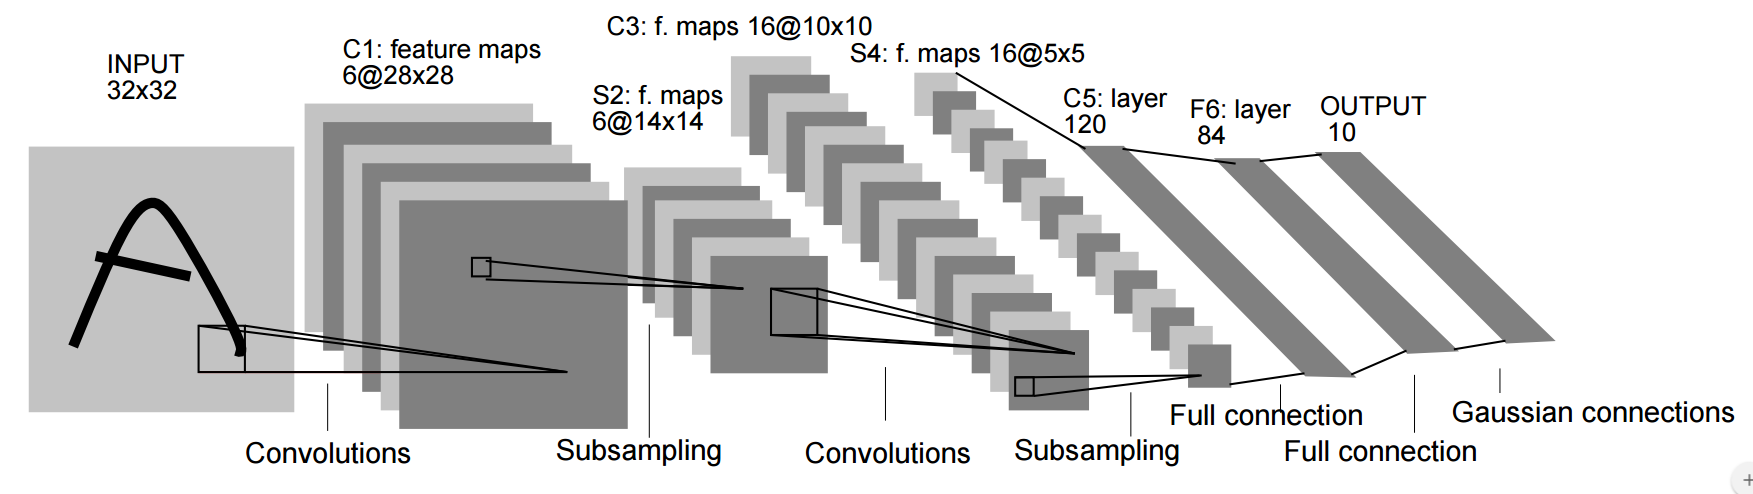
\includegraphics[width=0.7\textwidth]{images/images_lenet/LenetArquitectura.png}
  \caption{LeNet-5 Arquitecture}
  \label{Lenet5Arquitectura}
\end{figure}

The basic architecture of LeNet-5 is two convolutional layer, followed each one by a max pooling layer and then a fully-connected layer. This architecture could be visualized in figure \ref{Lenet5Arquitectura} where it is possible to visualize the input image dimensions across the layers and its final shape.\\

LeNet is a useful convolutional neural network that is usually used by beginners users to learn deep learning matter because its short architecture and it is implemented in lots of deep learning framework using it to explain the framework. Because of this, LeNet-5 has been used as basis of the project and to learn Theano and convolutional neural networks theory and implementation.\\

The code of LeNet in Python using Theano library, and its explanation, is openly available in \url{www.deeplearning.net}.\\

\subsection{LeNet-5 specifications}
The specifications of the downloaded LeNet code are the architecture of LeNet-5 used for starting to work with this project is formed by two convolutional layers of size 5x5 and with 20 kernels in the first convolutional layer and 50 in the second one, those are followed (each one) by a max pooling-layer of size 2x2. Those four layer are followed by a fully-connected layer with 500 neurons at the output.\\

The classifier which has been used is the logistic regression which is trained at the same time as the convolutional neural network. The activation function of the convolutional layers and the logistic regression is tanh. The learning rate used is 0.1 and the network runs by 200 epoch.\\

The cost function or loss that must be minimized during the training is the negative log-likelihood. LeNet-5 uses the stochastic gradient method with mini-batches (MSGD).\\

The data used is MNIST digit database, whose characteristics are described in section \ref{subsec:MNIST}. The data comes split in three subsets: training, testing and validating. Each subset is used for training, testing or validating respectively.\\

The data is not fed to the network in one go, each subset is grouped in smalls subsets called batches and whose size is chosen by user. In the code available of LeNet-5 the batch size is 500 samples. The network is fed by batches, so the size of the net depends on the batch size not the (train, test or validate) subset. In this example, the batch size, is the same for the three subsets. When the subset is divide into batches, if there are some samples that are not enough for a batch, those samples are not used.\\

The network train for a specified number of epoch. Each epoch has as many iterations as necessary to go through all batches of the train subset. The reason of using batches is to define the size of the network and because, usually, the quantity of samples used in deep learning is big (thousand, millions..) and too much memory would be need to build a network of its size and the computational resources available may not be enough.\\

As the MNIST digit database available with the code has 50000 samples for training, 10000 for testing and 10000 for validating, the number of batches for each subset (with 500 samples for each batch) is 100 for training, 20 for testing and 20 for validating

The training procedure is being realized for too many epochs as users has selected and returns the cost of the procedure. While the trianing is being running, the validation is calculated for each epoch and the validation returns the error of the procedure. The training cost and the validation error are used to know the behavior or the learning process of the network and how it generalizes with the purpose of choosing the best model.\\

The test is realized while the training is being executed, more specifically, when the validation has been realized and the results are the best obtained in the whole process until that iteration. The result that is used to compared with others classifiers or with others articles.\\

In addition to the number of epoch, other way to stop the training procedure is early-stopping, this method is used to avoid over fitting tracking the validation process \cite{Yoshua}. The decision of stopping the training depends on \textit{the patience} and is chosen by user.\\

%%%%% Creo que esto de aqui abajo no es necesario %%%%%%
%First of all in Lenet the data is loaded. The function that download the data check, firstly, if the data is not downloaded yet, if it downloaded it does not repeat the download. The data is downloaded split into train, test and validation subsets.\\

%After loading the data, the architecture is defined, the layers are called because they has been defined as objects, each kind of layer, one different object. There is a object for convolutional + maxpooling, another object for the hidden layers that is a fully connected layer, and the classifier used that is logistic regression. Each part of the code could be found in \url{www.deeplearning.net}\\

%After creating the structure, the functions of training, validating and testing are created as Theano functions.\\

%In a big while loop the training validation and testing is developed. The data is trained. Each mini-batch (that is a small quantity of that given by the user, it is used in order to not train or test all the data together because it would take too much computer resources) is trained and the weights and bias of each layer are updated. It is given a validation frequency, this parameters decides how many validations are produced. So the data is trained and validation, when a best score of validation is produced, the data is tested.\\

%The training would run for a number of epoch that the user has given or by a early-Stopping that has been developed by authors. The early-stopping combats over-fitting by monitoring the model's performance on a validation set.\\

\subsection{LeNet-5 Results}
While the training is being calculate, the weights are being update in each iteration. When A  model is selected or saved, weights are actually what is being chosen or saved. An example of weights is represented in figure \ref where twenty first weights at epoch 10 of the first convolutional layer are represented. So when its being trained, what the network is doing is adapting the weights to the input to get a good performance.\\

\begin{figure}[htb]
\centering
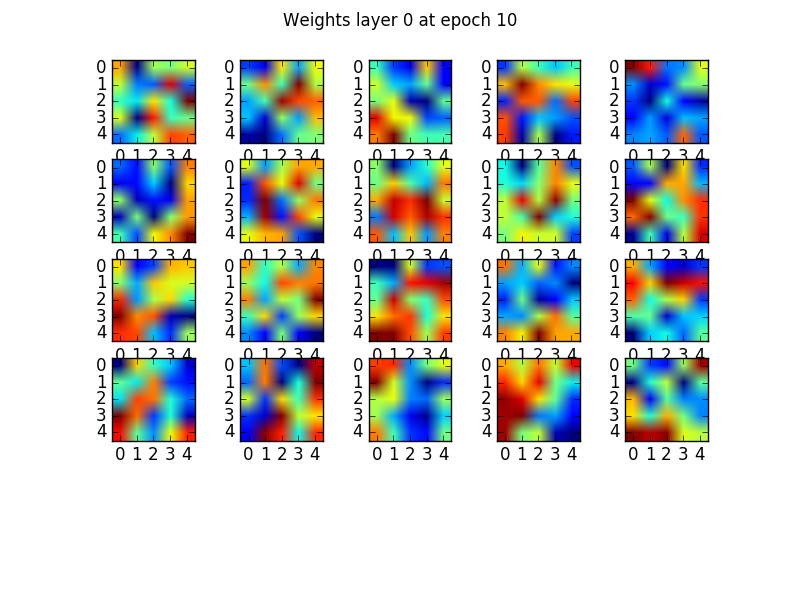
\includegraphics[width=0.7\textwidth]{images/images_lenet/w_layer0_epoch10.png}
\caption{Weights at epoch 10 of the first convolutional layer} \label{fig:weights_lenet}
\end{figure}

The training procedure returns the cost function in each iteration to evaluate the training behavior. The cost function at training obtained executing LeNet-5 is represented in figure \ref{fig:Lenetcost}, and its value decreases as the iterations rise converging in almost 0; this curve is the desired one for each training practice, because it is not oscillate abruptly and converges in a very low value logarithmically.\\

\begin{figure}[htb]
\centering
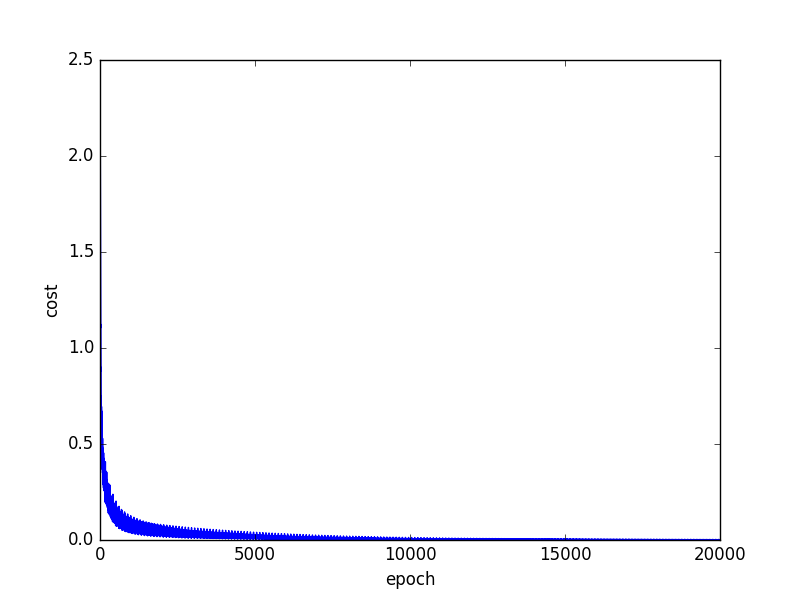
\includegraphics[width=0.7\textwidth]{images/images_lenet/cost_lenet.png}
\caption{Cost function at training running LeNet-5 with MNIST digit database.} \label{fig:Lenetcost}
\end{figure}

The error obtained at validation is represented in figure \ref{fig:Lenetresult}, where could be seen that the value decreases logarithmically too converging, approximately, in 1 (a low value) and this behavior of the curve is the desired in a validation process. The convergence value of the validation is not usually as much lower as the training convergence value, and the point where it starts to converge is later than in the training.\\

\begin{figure}[htb]
\centering
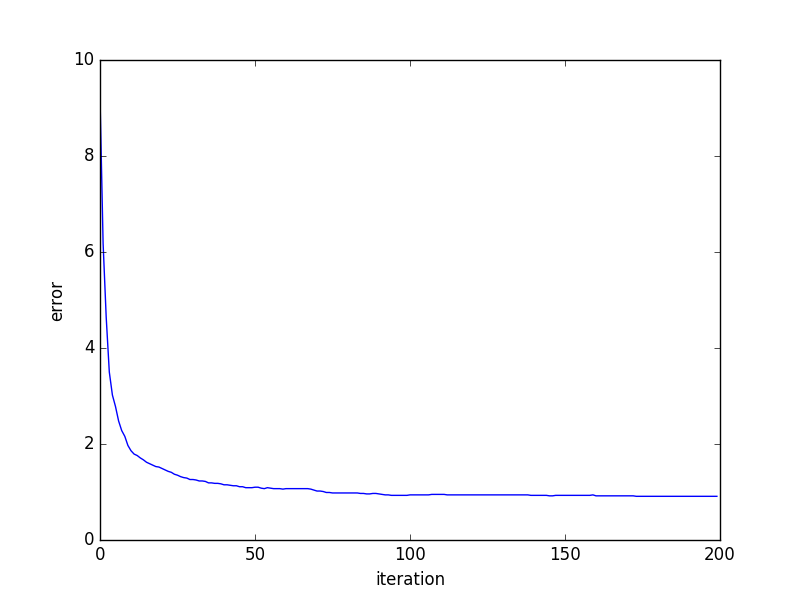
\includegraphics[width=0.7\textwidth]{images/ModificandoLenet/error_lenet.png}
\caption{Validation error obtained with LeNet-5 with MNIST digit database} \label{fig:Lenetresult}
\end{figure}

The test result has been calculated with the model of the iteration 18300 (epoch $37^{th}$), with a validation error of 0.91\%. The error rate obtained is 0.92\% what it means that 920 samples of 100000 of the testing subset are being misclassified.\\

%The neural network has beoen built in Python using Theano library. The %network has been based on the one exposed in \textit{Learn Convolutional %Neural Network for Face Anti-Spoofing} and \textit{LeNet}.\\

%The architecture of the network is formed by two convolutional layers which %is followed (each one) by a max-pool layer.The  last max-pool layer is %followed by a fully-connected layer which have sigmoidal activation %function.\\

%The rectified linear activation function (reLu) is used as activation %function of the convolutional layers. It has been used a normalized %distribution of weights and bias, the same which was implemented in LeNet: %weights are sampled randomly from a uniform distribution in the range [-1/%fan-in, 1/fan-in], where fan-in is the number of inputs of the previous %layer. The ReLu function that has been used is the one implemented in %theano as theano.tensor.nnet.relu.\\

%The number of kernels used in the conv layers are 48 and 96 of size 5x5, %the size of the max-pool layer is 2x2.\\

%The network is trained with the 70\% of the data, the 30\% is used to test. %From the 70\% of the training data, the 25\% is used to validation.\\


\subsection{Modifying LeNet}
Modifications has been made to LeNet-5 architecture. First the batch size has been changed and then the activation function, a normalization has been added o the weight initialization. The database used for those experiments is the MNIST digit database.\\

\subsubsection{Changing the batch size}
Two experiments have been developed in order to compare the results when the batch size is changed and how the network behavior change too with respect to LeNet-5 with the original batch size (500).\\

The first experiment is with 20 samples per batch. For the second experiment, the batch size used is 100. In both cases, the training process has been stopped by the early-stopping; at epoch $31^{th}$ has stopped the first experiment, because from epoch $16^{th}$ the error at validating was not being improved and for the second experiment, at $33^{th}$ epoch is when the early-stopping has finished the training.\\

The validation error for both experiments and the original LeNet are represented in figure \ref{figures:LENET-batches}. From images could be seen that the validation error in first epochs is lower (9 \% in the first experiment) than the validation error when the batch size is bigger. Whith the batch size equal to 20, the optimal test error rate has been obtained in the first $15^{th}$ epochs, the same error rate than in the original case (0.92\%), but for 100 samples per batch, it has not been possible to get to that error rate, the best test error rate has been 1.04\% at iteration 8500.\\

\begin{figure}[htb]
    \centering
	\subfigure[batch size = 500 (original size)]{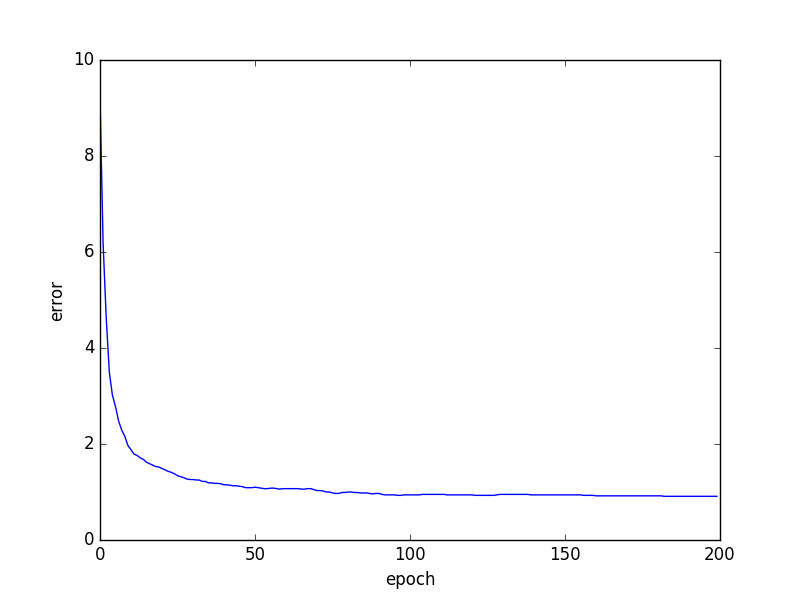
\includegraphics[width=0.47\textwidth]{images/images_lenet/lenet_batch/lenet_500batch_rror.png} }
	\subfigure[batch size = 20]{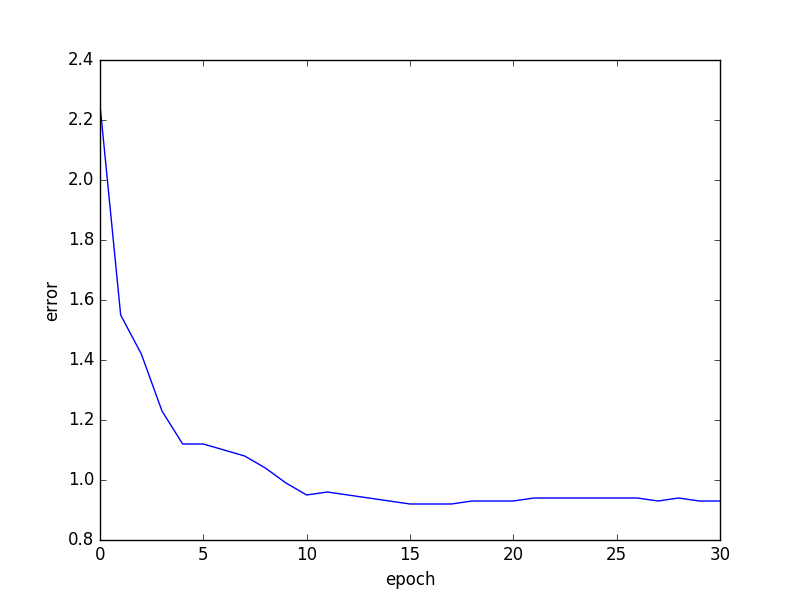
\includegraphics[width=0.47\textwidth]{images/images_lenet/lenet_batch/lenet_20batch_error.png} }
	\subfigure[batch size = 100]{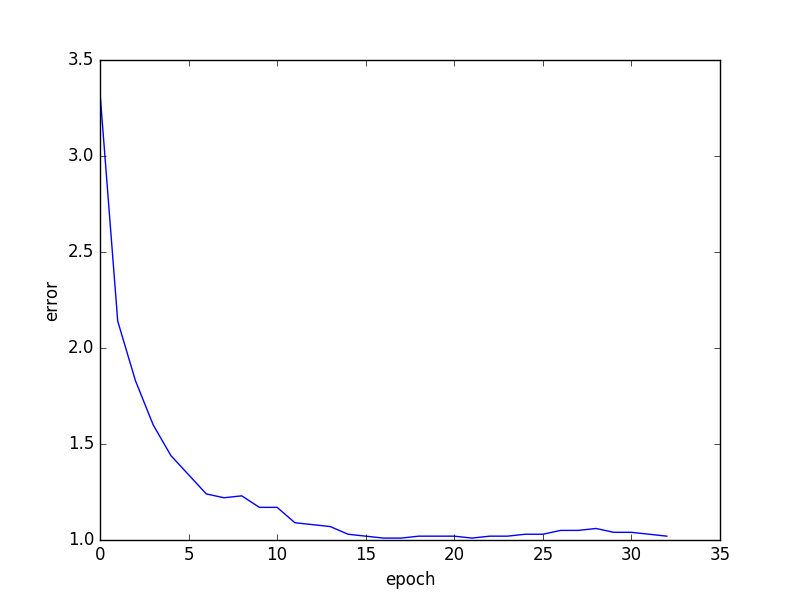
\includegraphics[width=0.47\textwidth]{images/images_lenet/lenet_batch/lenet_100batch_error.png} }

    \caption{Validation error in each epoch for different sizes of batches.} \label{figures:LENET-batches}
\end{figure}

%Each time we take a sample and update our weights it is called a mini-batch. Each time we run through the entire database, it's called an epoch. Batch size determines how many examples you look at before making a weight update. The lower it is, the noisier the training signal is going to be, the higher it is, the longer it will take to compute the gradient for each step. \url{http://stats.stackexchange.com/questions/140811/how-large-should-the-batch-size-be-for-stochastic-gradient-descent}.\\

Concluding, more epochs are necessary when the batch size is bigger because there are not enough updates in each epoch \cite{Yoshua}. Usually, the value of the batch size used is 32 \cite{Yoshua} and the choice, generally, is computational.\\

In figure \ref{figures:LENET-batches} the error in each epoch is represented  for 500 batch size, the original size, for a value of 20 and 100. In the original case, the error stars with a value of 9\% approx. with the batch size = 20 the error in the first iteration is about 2.4\%, and with a bunch of 100 images, the validation error is 3.5\%.\\

With the original size and size equal to 20, it is possible to get to the same minimum, the difference between those examples is that each one get to that conclusion into different epochs. With a batch size equal to 100, the code stopped because of the early-stop with a patience of 10000; it stop in epoch 33,while those epochs, it has been possible to get to a test error of 1.04\% in iteration 8500 when the validation error was 1.01\%, it has been running with put getting a better validation score for 17 epoch. With a batch size = 20, the code also has stopped earlier because of the same reason, but in that case it has been possible to get to the same minimum that with the original size; the epoch in which has stopped is 31, it has been running without getting a better validation score for 15 epochs.\\


%If the patience is increased from 10000 to 100000 for a batch size = 20 and equal to 100, results obtained are that for a value of 20, it has been running for 40 epoch, having the same results that the one obtained with a patience of 10000.\\

%For a value of 100 with the patience increased to 100000, the results are not the same as the one obtained the patience equal to 10000. In this occasion, the results are better than in the original one; The code has run for 258,08 minutes and for 200 epochs. The result obtained was better than in the original one has it has said. In epoch 51 has gotten a validation error of  1 \% and the error test has been 0,89\%, from this point, the test error that has been calculated five more times, has been increasing until get the value 0,85\% in iteration 55500, epoch number 111, the validation error obtained has been 0,95\%. From this epoch until number 200, the network has not had any better result.\\

%In figure X it is possible to see the error function for those two examples. It could be seen that the example with batch size = 20 has just run for 40 epoch and the good results of the example with batch size = 100, remembering that the patience has been increased from 10000 to 100000.\\


\subsubsection{Changing activation function, normalization and weights initialization}
As the same way as the batch has been changed and its results has been compared in the previous subsection, the activation function has been changed, a normalization layer has been added and weights initialization has been changed.\\

LeNet-5 does not use any normalization layer, but in this experiment from the different normalization availables (batch normalization, local normalization, ...) Local Response normalization has been added after the max-pooling layers.\\

The activation function used in LeNet-5 is tanh, it has been changed to rectified linear unit (ReLu) activation function.\\

With respect to the weight initialization, in LeNet, for the convolutional layers and the fully connected layer,  a normalized initialization \cite{XavierInitialization} is used:

\begin{equation}
  W \sim U [- \frac{\sqrt{6}}{\sqrt{n_{j}+n_{j+1}}},\frac{\sqrt{6}}{\sqrt{n_{j}+n_{j+1}}}]
\end{equation}

Where $n_{j}$ is the number of neuron of the current layer and $n_{j}$ is number of neurons of the following layers. In this experiment, this initialization has been changed to a weight initialization with a Gaussian distribution.\\

Above the details of each experiment are described:\\

\begin{itemize}
\item{Experiment 1: using Local Response Normalization (LRN) In which a normalization has been carried out in the convolutional-max pooling layers.}
\item{Experiment 2: using ReLu as activation function:} The activation function tanh has been substituted by ReLu activation function in convolutional and fully connected layers.
\item{Experiment 3: using ReLu and LRN}: The activation function used is ReLu and LRN has been used as  normalization layer.
\item{Experiment 4: changing weights initialization}: Weights initialization has been changed by Gaussian. In which mean value that has been used is 0 and std is 0.01. Weights initialization has been changed in convolutional and fully connected layers. Also, bias initialization has been changed by ones.
\end{itemize}

%Using Local Response Normalization we want to detect high frequency features with a large response. If we normalize around the local neighborhood of the excited neuron, it becomes even more sensitive as compared to its neighbors.[\url{https://prateekvjoshi.com/2016/04/05/what-is-local-response-normalization-in-convolutional-neural-networks/}].\\

First, the cost of training process are going to be visualized with the original cost train, without modifying LeNet). In figure \ref{fig:CostModLeNet} is represented. Also the validation error (validation cost*100) could be visualized in figure \ref{fig:CostModLeNet}. The network has been running for 200 epochs.\\

\begin{figure}[htb]    \centering
	\subfigure[Original LeNet]{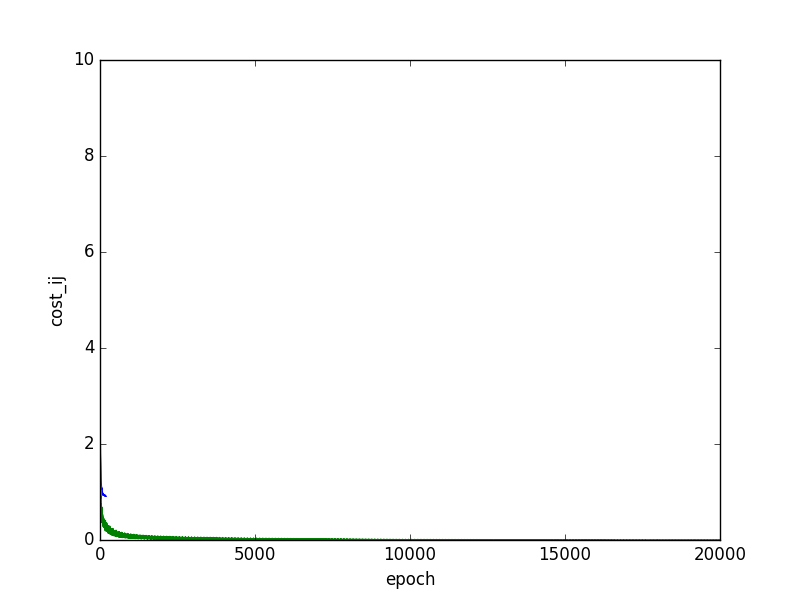
\includegraphics[width=0.42\textwidth]{images/ModificandoLenet/cost_lenet.png}\label{fig:cost_lenet} }
	\subfigure[Experiment 1: using LRN]{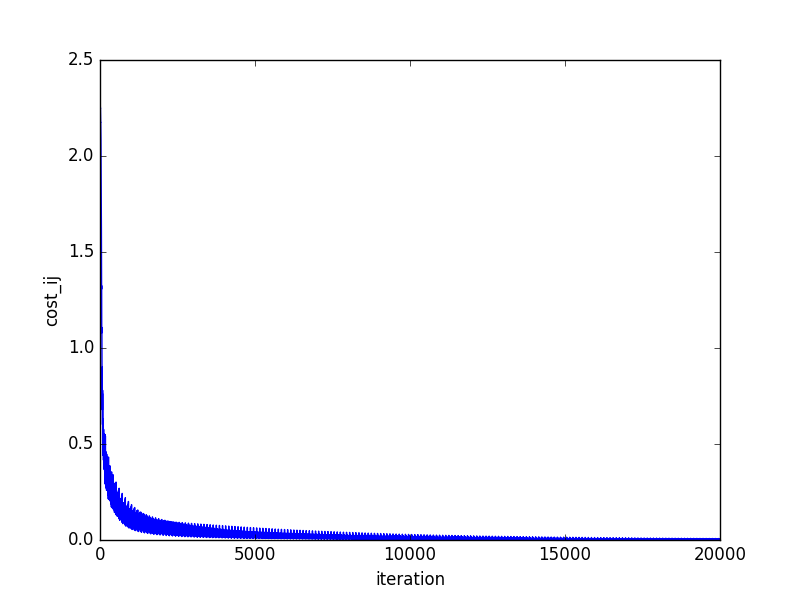
\includegraphics[width=0.42\textwidth]{images/ModificandoLenet/cost_lenet_LRN.png}}
	\subfigure[Experiment 2: using ReLu]{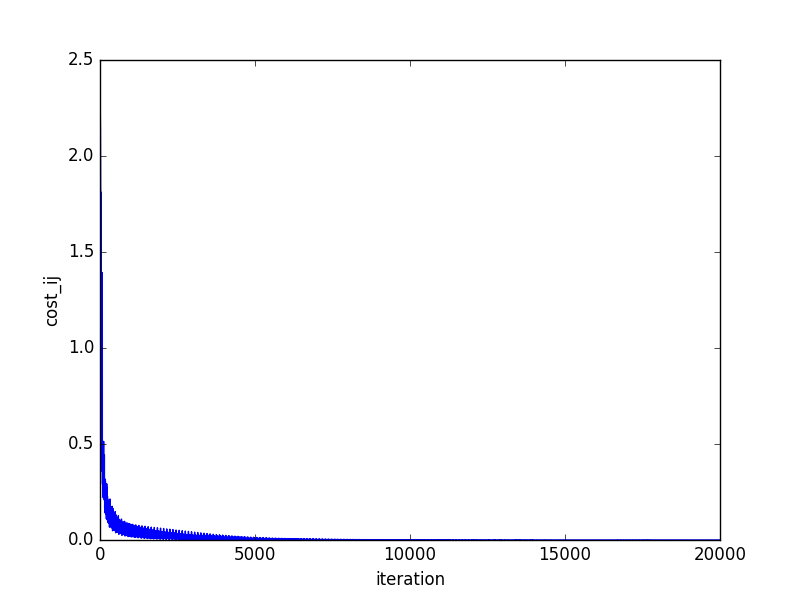
\includegraphics[width=0.42\textwidth]{images/ModificandoLenet/cost_lenet_relu.png}}
	\subfigure[Experiment 3: using ReLu and LRN]{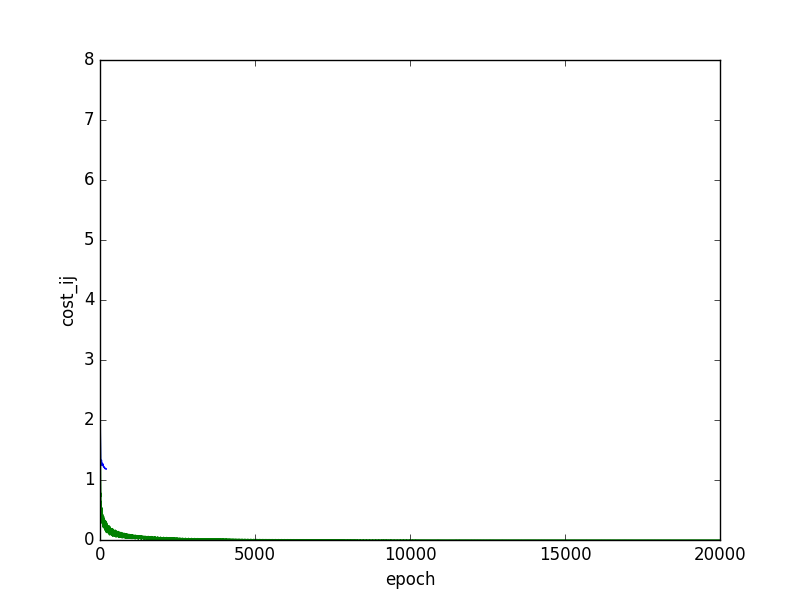
\includegraphics[width=0.42\textwidth]{images/ModificandoLenet/cost_lenet_relu_lrn.png}}
	\subfigure[Experiment 4: using Gaussian weights init.]{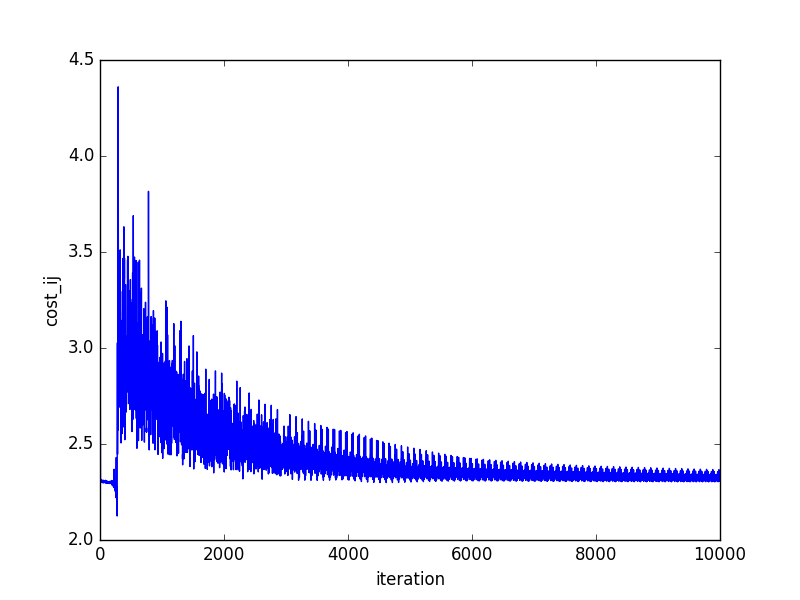
\includegraphics[width=0.42\textwidth]{images/ModificandoLenet/cost_lenet_gausianInit.png} \label{fig:cost_gaus_lenet}}
    \caption{Cost function of Lenet and Lenet Modified.} \label{fig:CostModLeNet}
\end{figure}

Visualizing the loss during the training, could be affirmed that the network with Gaussian initialization is in a local minimum because the loss has converged as could be seen in figure \ref{fig:cost_gaus_lenet}. The loss of LeNet without being modified (figure  \ref{fig:cost_lenet}) is the one whose oscillation at training is less than others.\\

\begin{figure}[htb]    \centering
	\subfigure[Original LeNet]{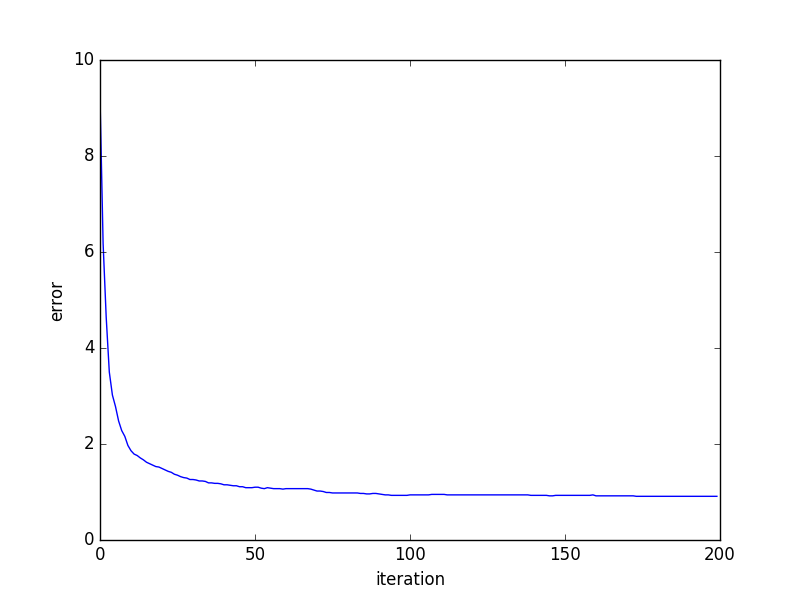
\includegraphics[width=0.42\textwidth]{images/ModificandoLenet/error_lenet.png}\label{fig:error_lenet} }
	\subfigure[Experiment 1: using LRN]{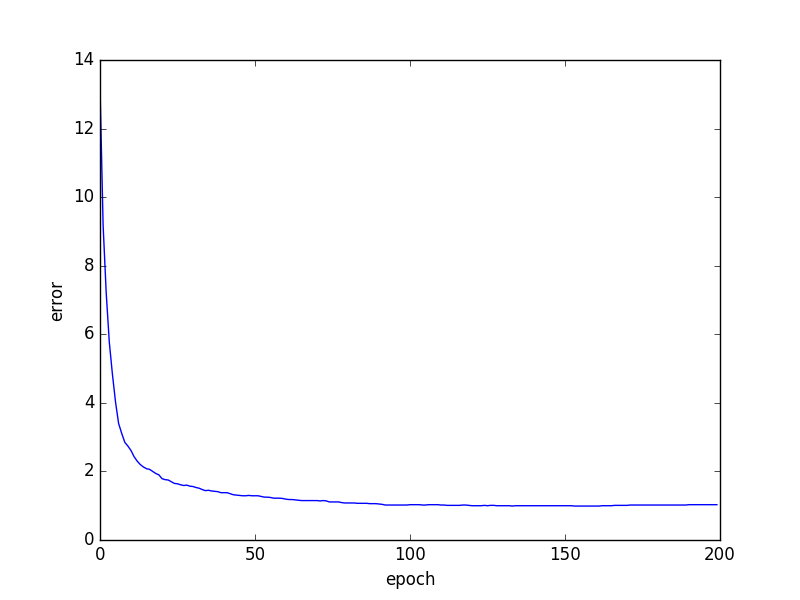
\includegraphics[width=0.42\textwidth]{images/ModificandoLenet/error_lenet_LRN.png}}
	\subfigure[Experiment 2: using ReLu]{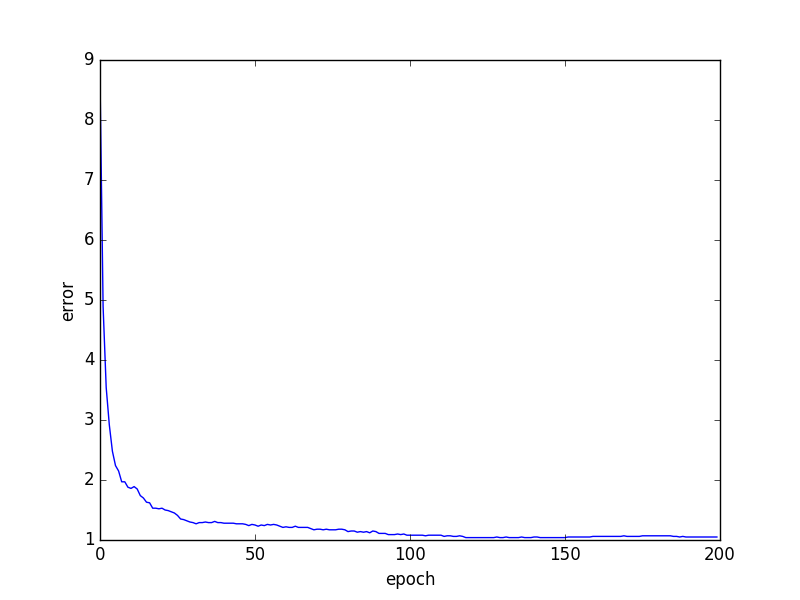
\includegraphics[width=0.42\textwidth]{images/ModificandoLenet/error_lenet_relu.png}}
	\subfigure[Experiment 3: using ReLu and LRN]{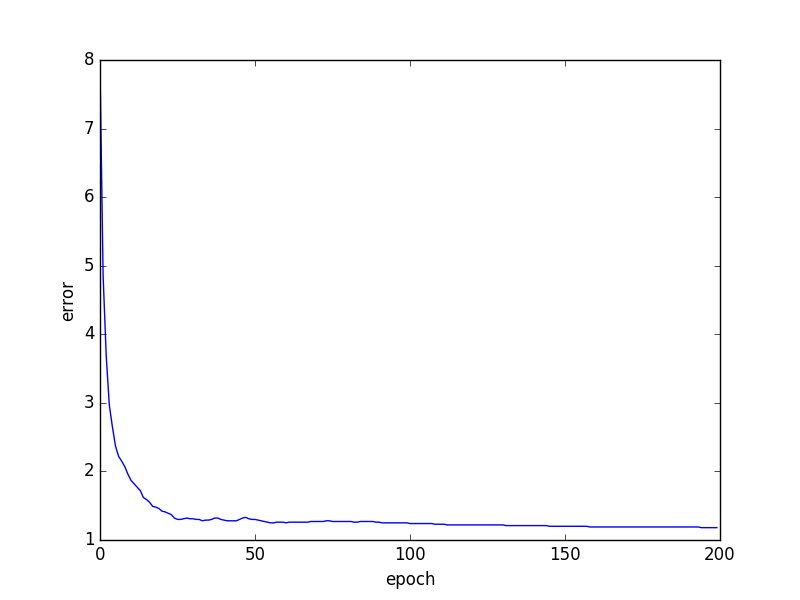
\includegraphics[width=0.42\textwidth]{images/ModificandoLenet/error_lenet_relu_lrn.png}}
	\subfigure[Experiment 4: using Gaussian weights init.]{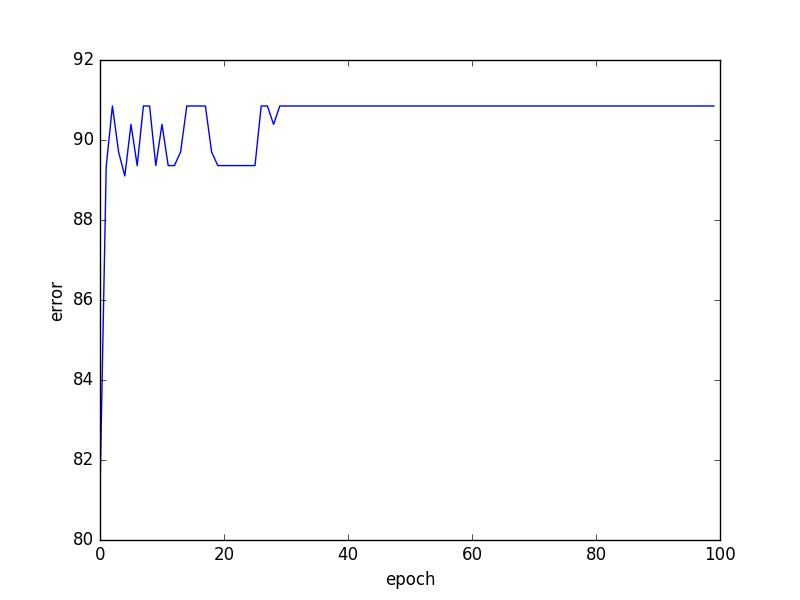
\includegraphics[width=0.42\textwidth]{images/ModificandoLenet/error_frav_gausianInit.png} \label{fig:error_gaus_lenet}}
    \caption{Valid error of Lenet and Lenet Modified.} \label{fig:ErrorModLeNet}
\end{figure}

About the error at validation, visualizing the graphs in figure \ref{fig:CostModLeNet}, it is very similar the curve for original LeNet-5, LeNet-5 with ReLu, LeNet-5 with LRN and LeNet-5 with LRN and ReLu.\\

The results obtained, at testing, have been the following ones:

\begin{itemize}
\item{Original LeNet}: Best validation score of 0.91 \% obtained at iteration 17400, with test performance 0.92\%.
\item{Experiment 1: using Local Response Normalization}: Best validation score of 0.99 \% obtained at iteration 13400, with test performance 1.6 \%.
\item{Experiment 2: using ReLu as activation function}:Best validation score of 1.04 \% obtained at iteration 11900, with test performance 2.4\%.
\item{Experiment 3: using ReLu and LRN}: Best validation score of 1.18 \% obtained at iteration 19500, with test performance 1.08 \%.
\item{Experiment 4: Gaussian weight initialization}: Best validation score of 81.22\% obtained at iteration 100, with test performance 80.90\%.
\end{itemize}

The best configuration for the network is the original one. With Gaussian initialization, the network does not find a local minimum in such a sort of time. Using LRN and ReLu, test result is closer to the obtained with LeNet original, but not as good as the last one. Changing the activation function has not been a good change. Not taking into account original LeNet, the best test performance has been obtained with 1,08\% using ReLu and LRN, but the best validation error is 0,99\% obtained using just LRN. The values are close of the modifications, but the modification of Gaussian weight initialization.\\

\clearpage
\section{Start working with Faces databases}
Once LeNet-5 architecture has been understanding, the used database is changed because the final goal is using a convolutional neural network with different faces databases.\\

\subsection{Using Labeled Faces in the Wild}
With the purpose of reading and working with face images, the Labeled Faces in the Wild (LFW) database is used. Because of that, a script has been developed where images are precessed. All images are pseudo-randomized and grouped in training set (49\% of the total database), testing test (30\% of the total data) and validating set (21\% of the data).\\

To split the data, train\_test\_split function from sklearn.cross\_validation has been used. This function pseudo-randomize the data, so you can repeat the randomized split data in the same way assigning the same seed to the function.\\

For the next experiment, 500 samples are used for each batch, so 13 batches are going to be used for training, 6 for validation and 6 for testing. Images has been resized to 28x28 size, as MNIST digit database available with the code. \\

The parameters has not been changed, but the number of epoch that has been decreased to 12, and the number of neurons at the output of the logistic regression that has been changed from 10 to 5748 (the number of classes or different people).\\

%\begin{itemize}
%\item $learning_rate=0.1, n_epochs=12, nkerns=[20, 50], batch_size=500$
%\item  T.tanh activation function
%\item rng = numpy.random.RandomState(23455)
%\item kernel size = [5,5]
%\item images resized to 28x28
%\item 12 epoch
%\item The number of neurons at the input of the regression class is 10000, and the number of neurons at the output is 5748 (Number of people).
%\end{itemize}
The results obtained are not good, because of the fact that the network has not been optimized to this purpose, the number of epoch should be more and for each class there are a few samples and should be much more.\\

\begin{figure}[htb]
\centering
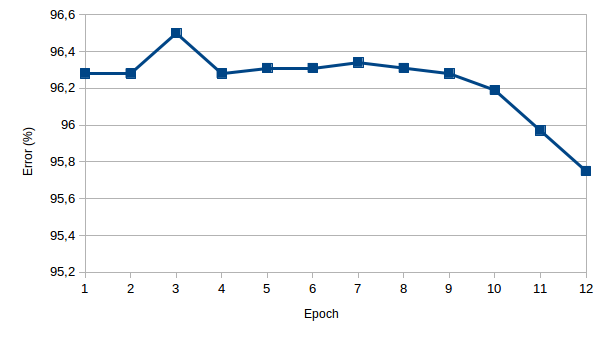
\includegraphics[width=0.7\textwidth]{images/epoch_LFW.png}
\caption{Error of Lenet using LFW.} \label{fig:LENETLFW}
\end{figure}

Figure \ref{fig:LENETLFW} represents the validation error \% in each epoch, and it could be seen that in the last epoch, the error is the smallest one, and the test error in that point is 95.125000 \%, a really high error rate because of the bag learning procedure.\\

\subsubsection{Changing learning rate}
Despite the fact that the configuration of the networks is not to this database, learning rate is going to be changed so it is possible to know how it affects.\\

In order to know how the net works with different learning rates, it has been changed to 0.001 and the number of epoch has been raised to 50.\\

The error at validating in each epoch could be seen in figure \ref{fig:LENETLFWerror0-001} , where it is shown that the net does not learn because the learning rate is too small and it would need more epochs. The cost function at training of the training could be seen in figure \ref{fig:LENETLFWcost0-001}, where the cost it has been reducing during epochs, but it has not been reduced significantly, from 8.7 to 8.1.\\

\begin{figure}[htb]
\centering
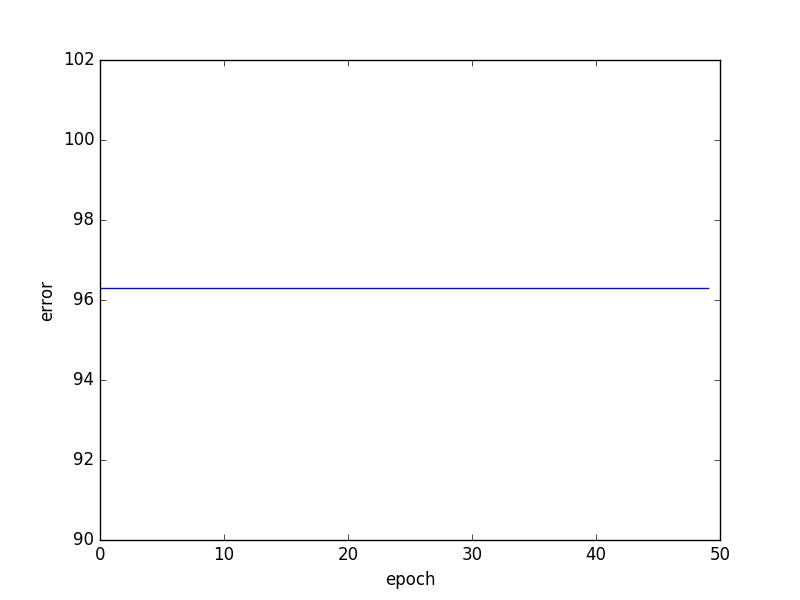
\includegraphics[width=0.7\textwidth]{images/LFW_learningrate/error_0_001.png}
\caption{Error of LeNet-5 using LFW with a learning rate of 0.001.} \label{fig:LENETLFWerror0-001}
\end{figure}

\begin{figure}[htb]
\centering
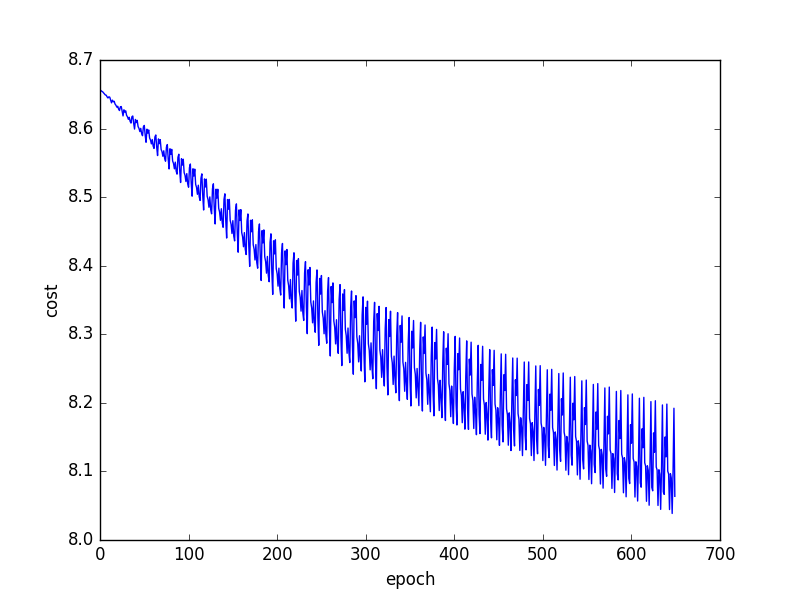
\includegraphics[width=0.7\textwidth]{images/LFW_learningrate/cost_0_001.png}
\caption{Cost of Lenet using LFW with a learning rate of 0.001.} \label{fig:LENETLFWcost0-001}
\end{figure}

A 97,73\% error of test performance has been gotten, which has been obtained in iteration 13. \\

The conclusion is the learning rate is too small to this configuration of the net and the data given.\\

If the learning rate is increased to 0.01: Best validation score of 96.266667 \% obtained at iteration 481, with test performance 95.733333 \%\\

\begin{figure}[htb]
\centering
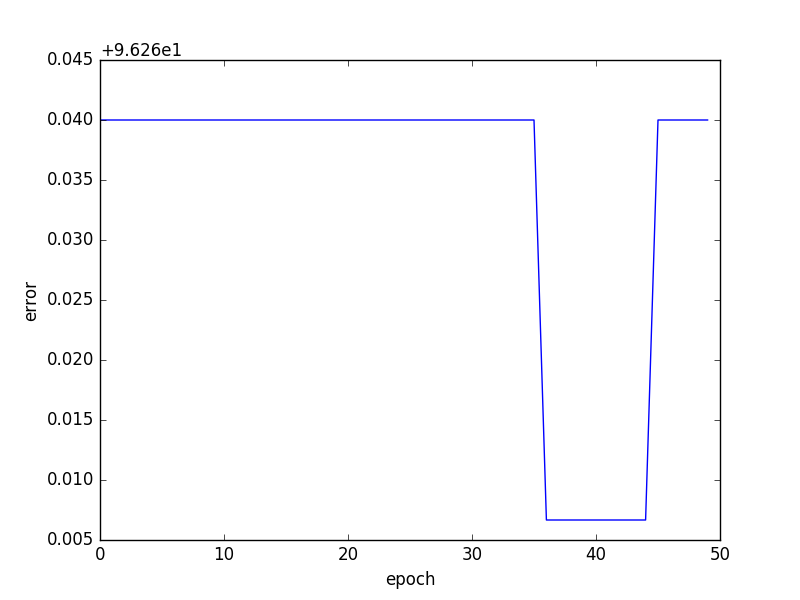
\includegraphics[width=0.7\textwidth]{images/LFW_learningrate/error_0_01.png}
\caption{Error of Lenet using LFW changing learning rate to 0.01.} \label{fig:LENETLFW_lr0_01}
\end{figure}

If learning rate is increased to 0.1:Best validation score of 96.300000 \% obtained at iteration 13, with test performance 95.733333 \%\\

\begin{figure}[htb]
\centering
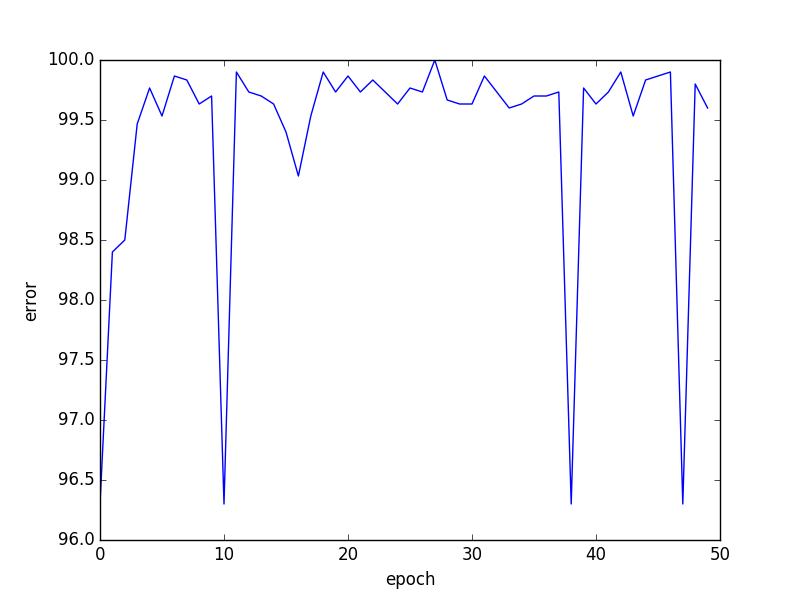
\includegraphics[width=0.7\textwidth]{images/LFW_learningrate/error_0_1.png}
\caption{Error of Lenet using LFW changing learning rate to 0.1.} \label{fig:LENETLFW_lr0_1}
\end{figure}

If learning rate = 0.5 Best validation score of 96.3 \% obtained at iteration 143, with test performance 95.73\% \\

\begin{figure}[htb]
\centering
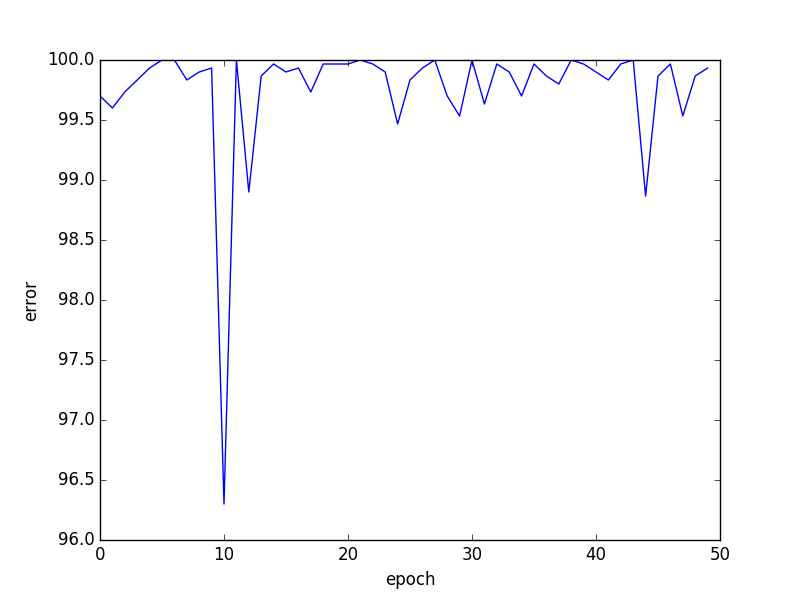
\includegraphics[width=0.7\textwidth]{images/LFW_learningrate/error_0_5.png}
\caption{Error of Lenet using LFW changing learning rate to 0.5.} \label{fig:LENETLFW_lr0_5}
\end{figure}

In conclusion, if the learning rate is too big, the network do not get a optimal minimum and if the learning rate is too small it takes too mch iteration to learn or getting to to optimal minimum.\\


\subsubsection{Changing convolutional parameters}
Convolutional layers are built with the Theano function \textit{theano.tensor.nnet.conv2d}. The size of convolutional layers depends on the number of filters that users would like, the dimension of images, it is not possible to use the same convolutional layer for 3d images (rgb) than grey scale images (1 dimension), and also depends on the high and width user would like to give.\\

The output of a convolutional layer depends on the size of the filter and the size of input images. At the output, a new bunch of images are created from the input images and the characteristics of the layer.\\

Also, it is important to consider the batch size, because the layer is not fed by a individual image; the layer is fed by the bunch of images.\\

Lets have a bit of fun with convolutional layers, the number of filters and the size of them it is going to be changed. A learning rate of 0.1 is going to be used for 50 epoch.\\

In the first example, the number of filters of the first layer is going to be increased from 20 to 40, and the number of the second layer from 40 to 60.

In figure \ref{fig:LENETLFW_ker1} could be seen the error which has been gotten in each epoch, where the best vest validation score of 94.9\% has been obtained at iteration 559, with test performance 95\%.

\begin{figure}[htb]
\centering
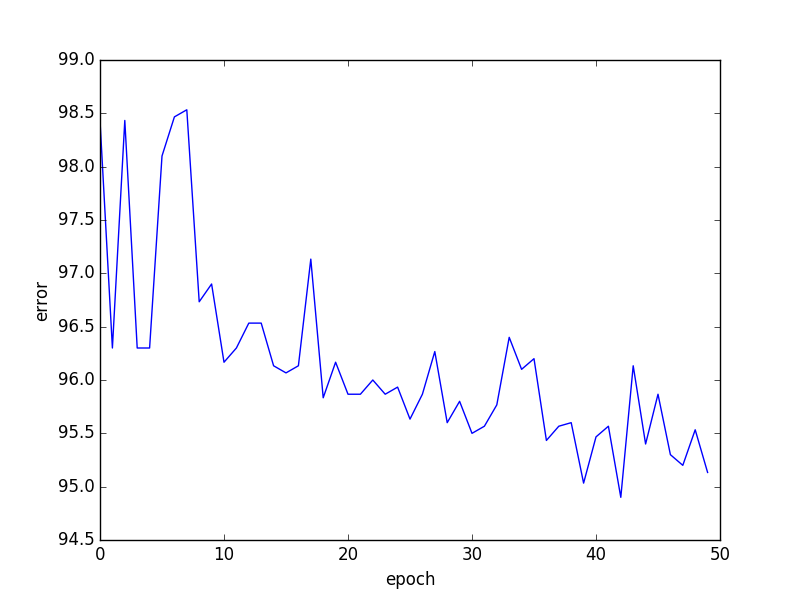
\includegraphics[width=0.7\textwidth]{images/LFW_layers/error_conv_40_60.png}
\caption{Error of Lenet using LFW changing number of kernels in example 1.} \label{fig:LENETLFW_ker1}
\end{figure}

If the number of filters has been increased, the time that the code takes to run is increased significantly. Also, the results of the network changes, this is a parameter that should have in consideration.\\

Also, it is possible to modify the filter shape, in the previous examples, the size of both kernels were 5x5, in this example, the second one, the first convolutional layer would have a filter size of 3x3, the second one would keep its original size.\\

\begin{figure}[htb]
\centering
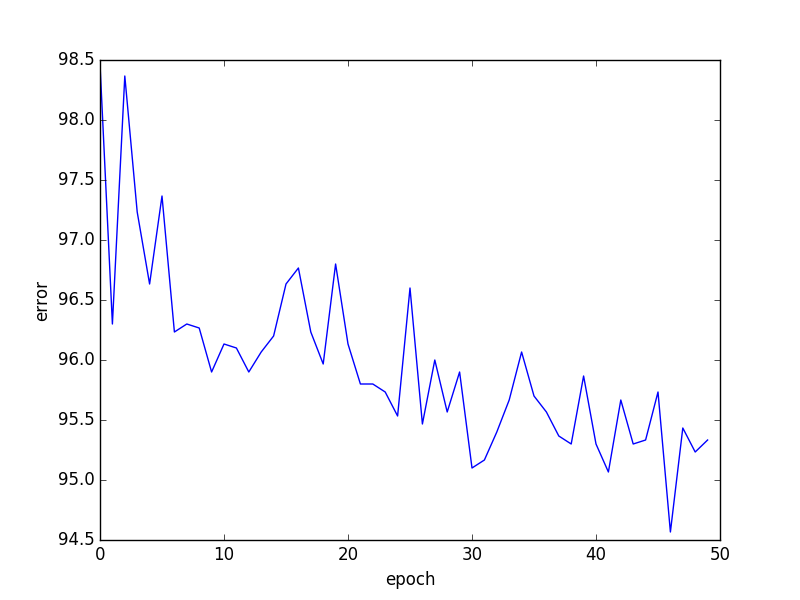
\includegraphics[width=0.7\textwidth]{images/LFW_layers/error_conv_40_60_2.png}
\caption{Error of Lenet using LFW changing number of kernels and the filter size in example 2.} \label{fig:LENETLFW_ker2}
\end{figure}

It is interesting seeing how the error of the network has been improved when the number of kernels has been changed and, in this example, has been improved too when the size of the filter has been changed.\\

The error in each epoch of this example could be seen in figure \ref{fig:LENETLFW_ker2}, where the best validation score obtained has been 94.567\% error iteration 611, with test performance error 93.967\%.\\

In order to see the difference between using a big size filter and one of a small size, in the next example, third example, 40 and 60 kernels are going to be used, and the size of each one is 3 and 10 for layer 0 and layer 1 respectively. In epoch number 40, the weighs of each layer has been saved and in figure X are represented. At irst sight, it is possible to see that with a big size.\\

\begin{figure}[htb]
\centering
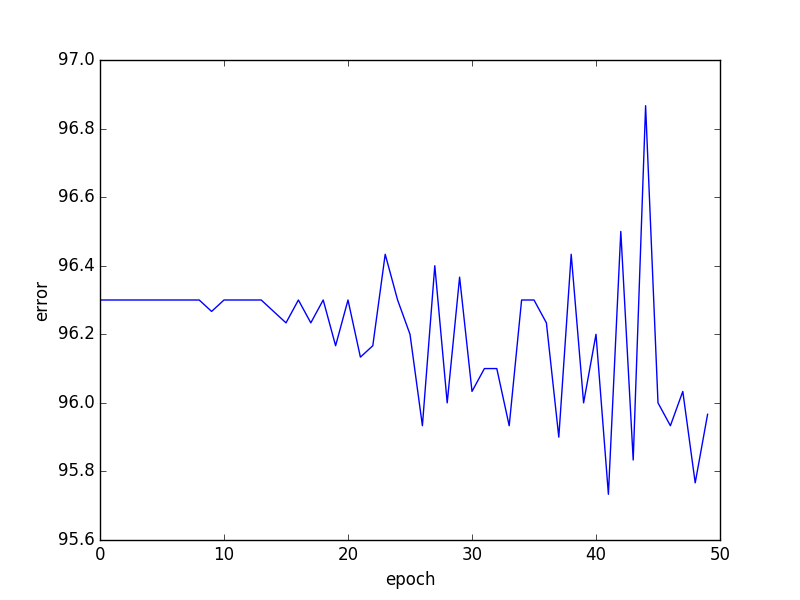
\includegraphics[width=0.7\textwidth]{images/LFW_layers/error_conv_40_60_3.png}
\caption{Error of Lenet using LFW changing number of kernels and the filter size in example 3.} \label{fig:LENETLFW_ker3}
\end{figure}

Also, it is possible to see the output at the convolutional layer, in figure \ref{fig:LENETLFW_ker4}, the first 25 output images are shown for both layers.\\

\begin{figure}[htb]
\centering
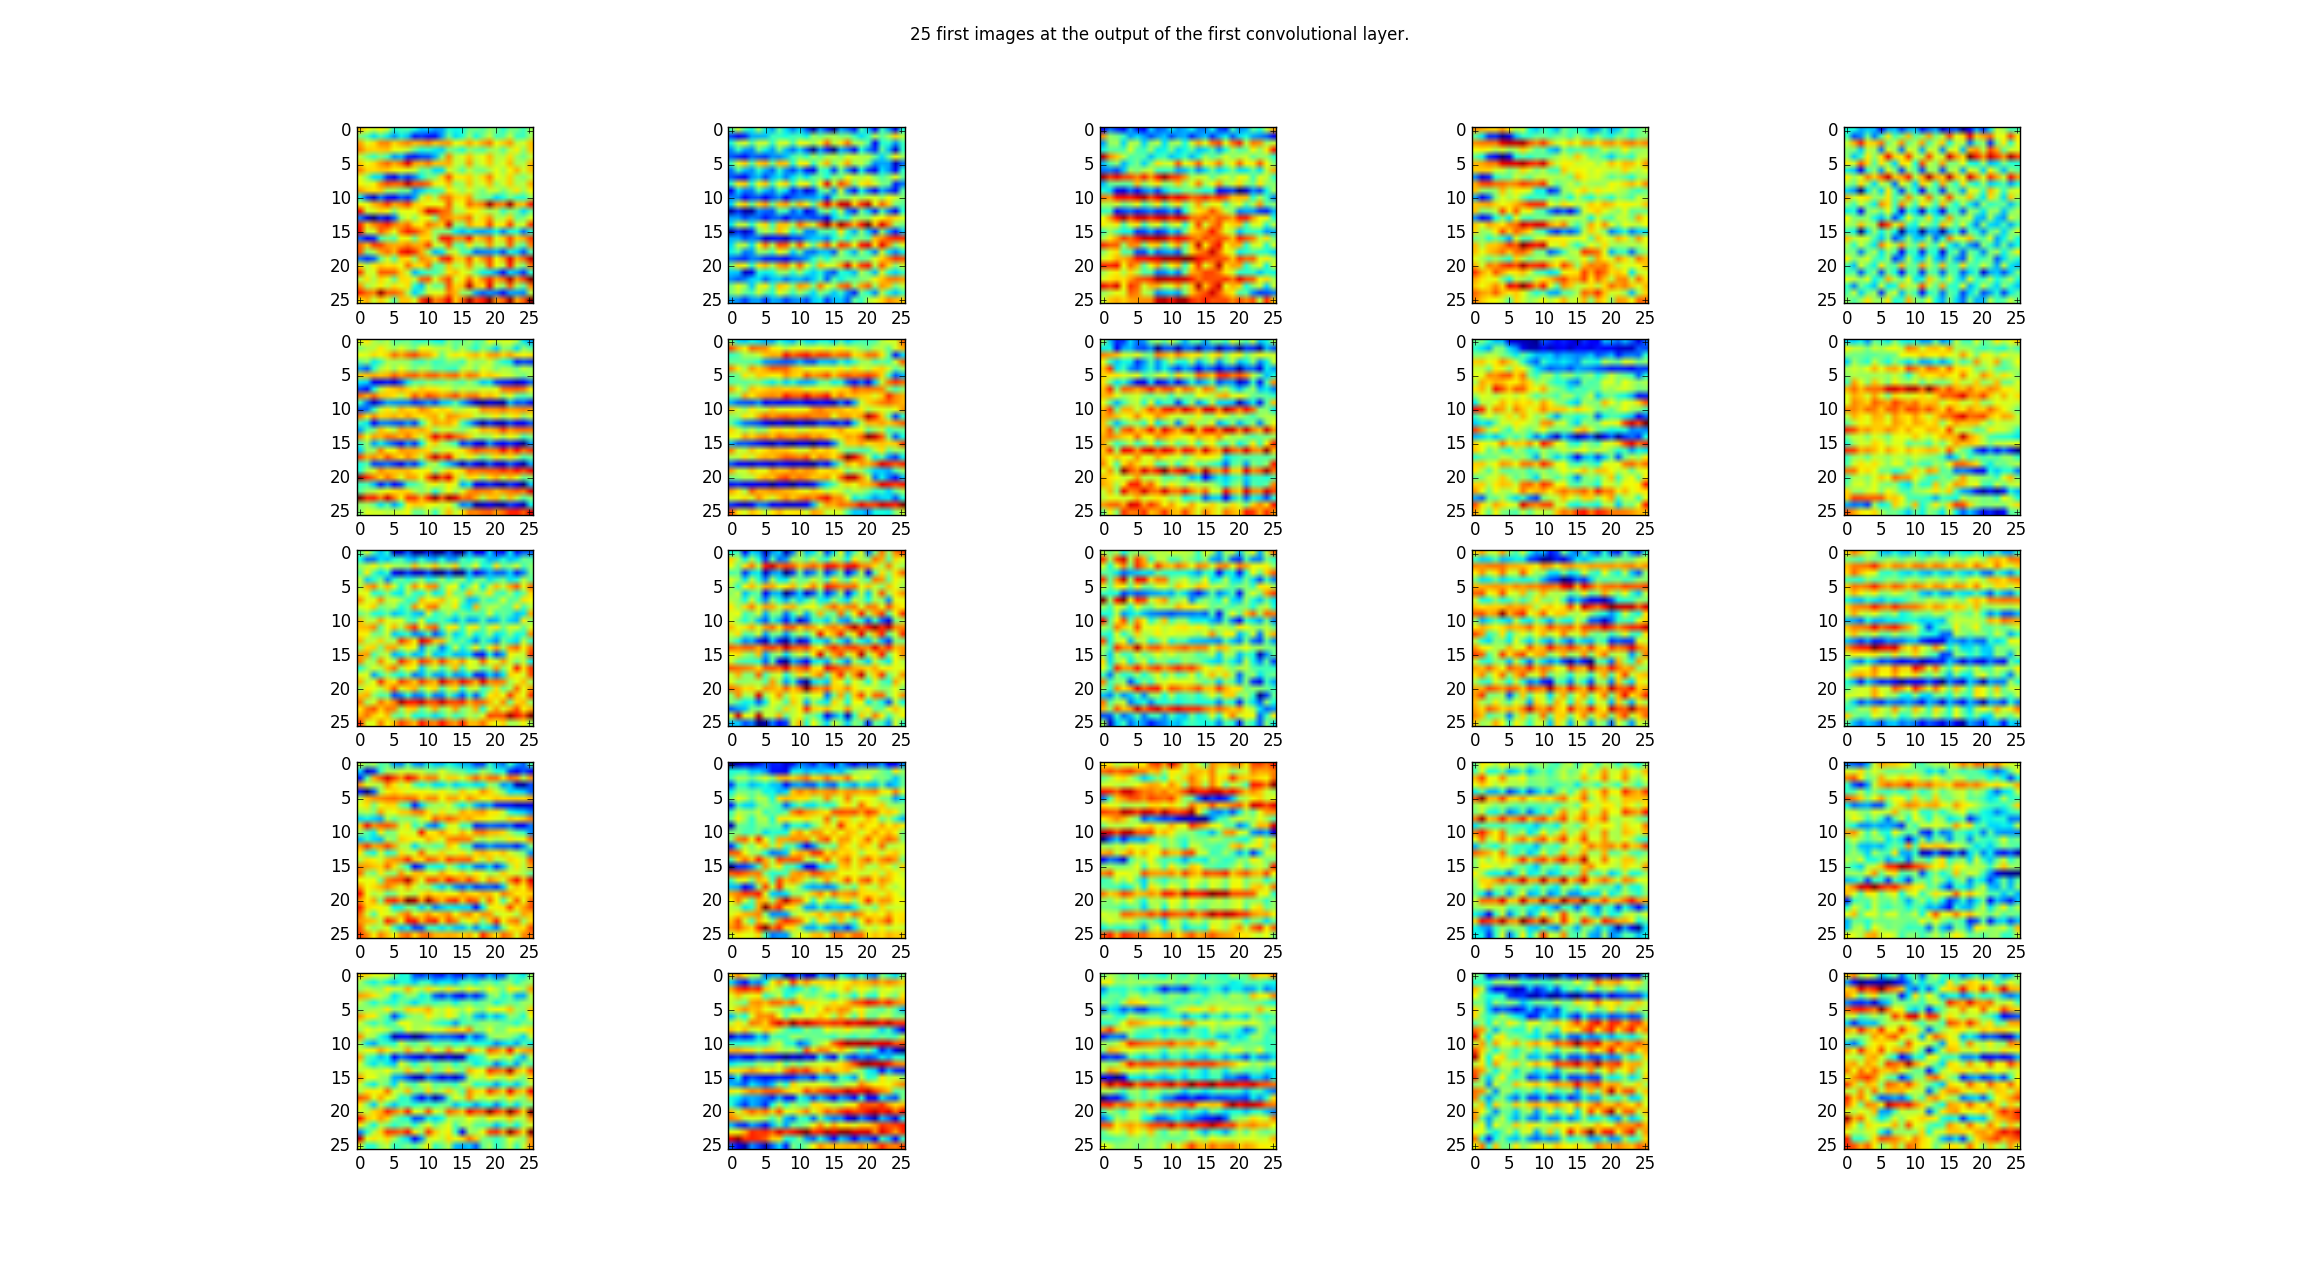
\includegraphics[width=1.4\textwidth]{images/LFW_layers/conv_0_out.png}
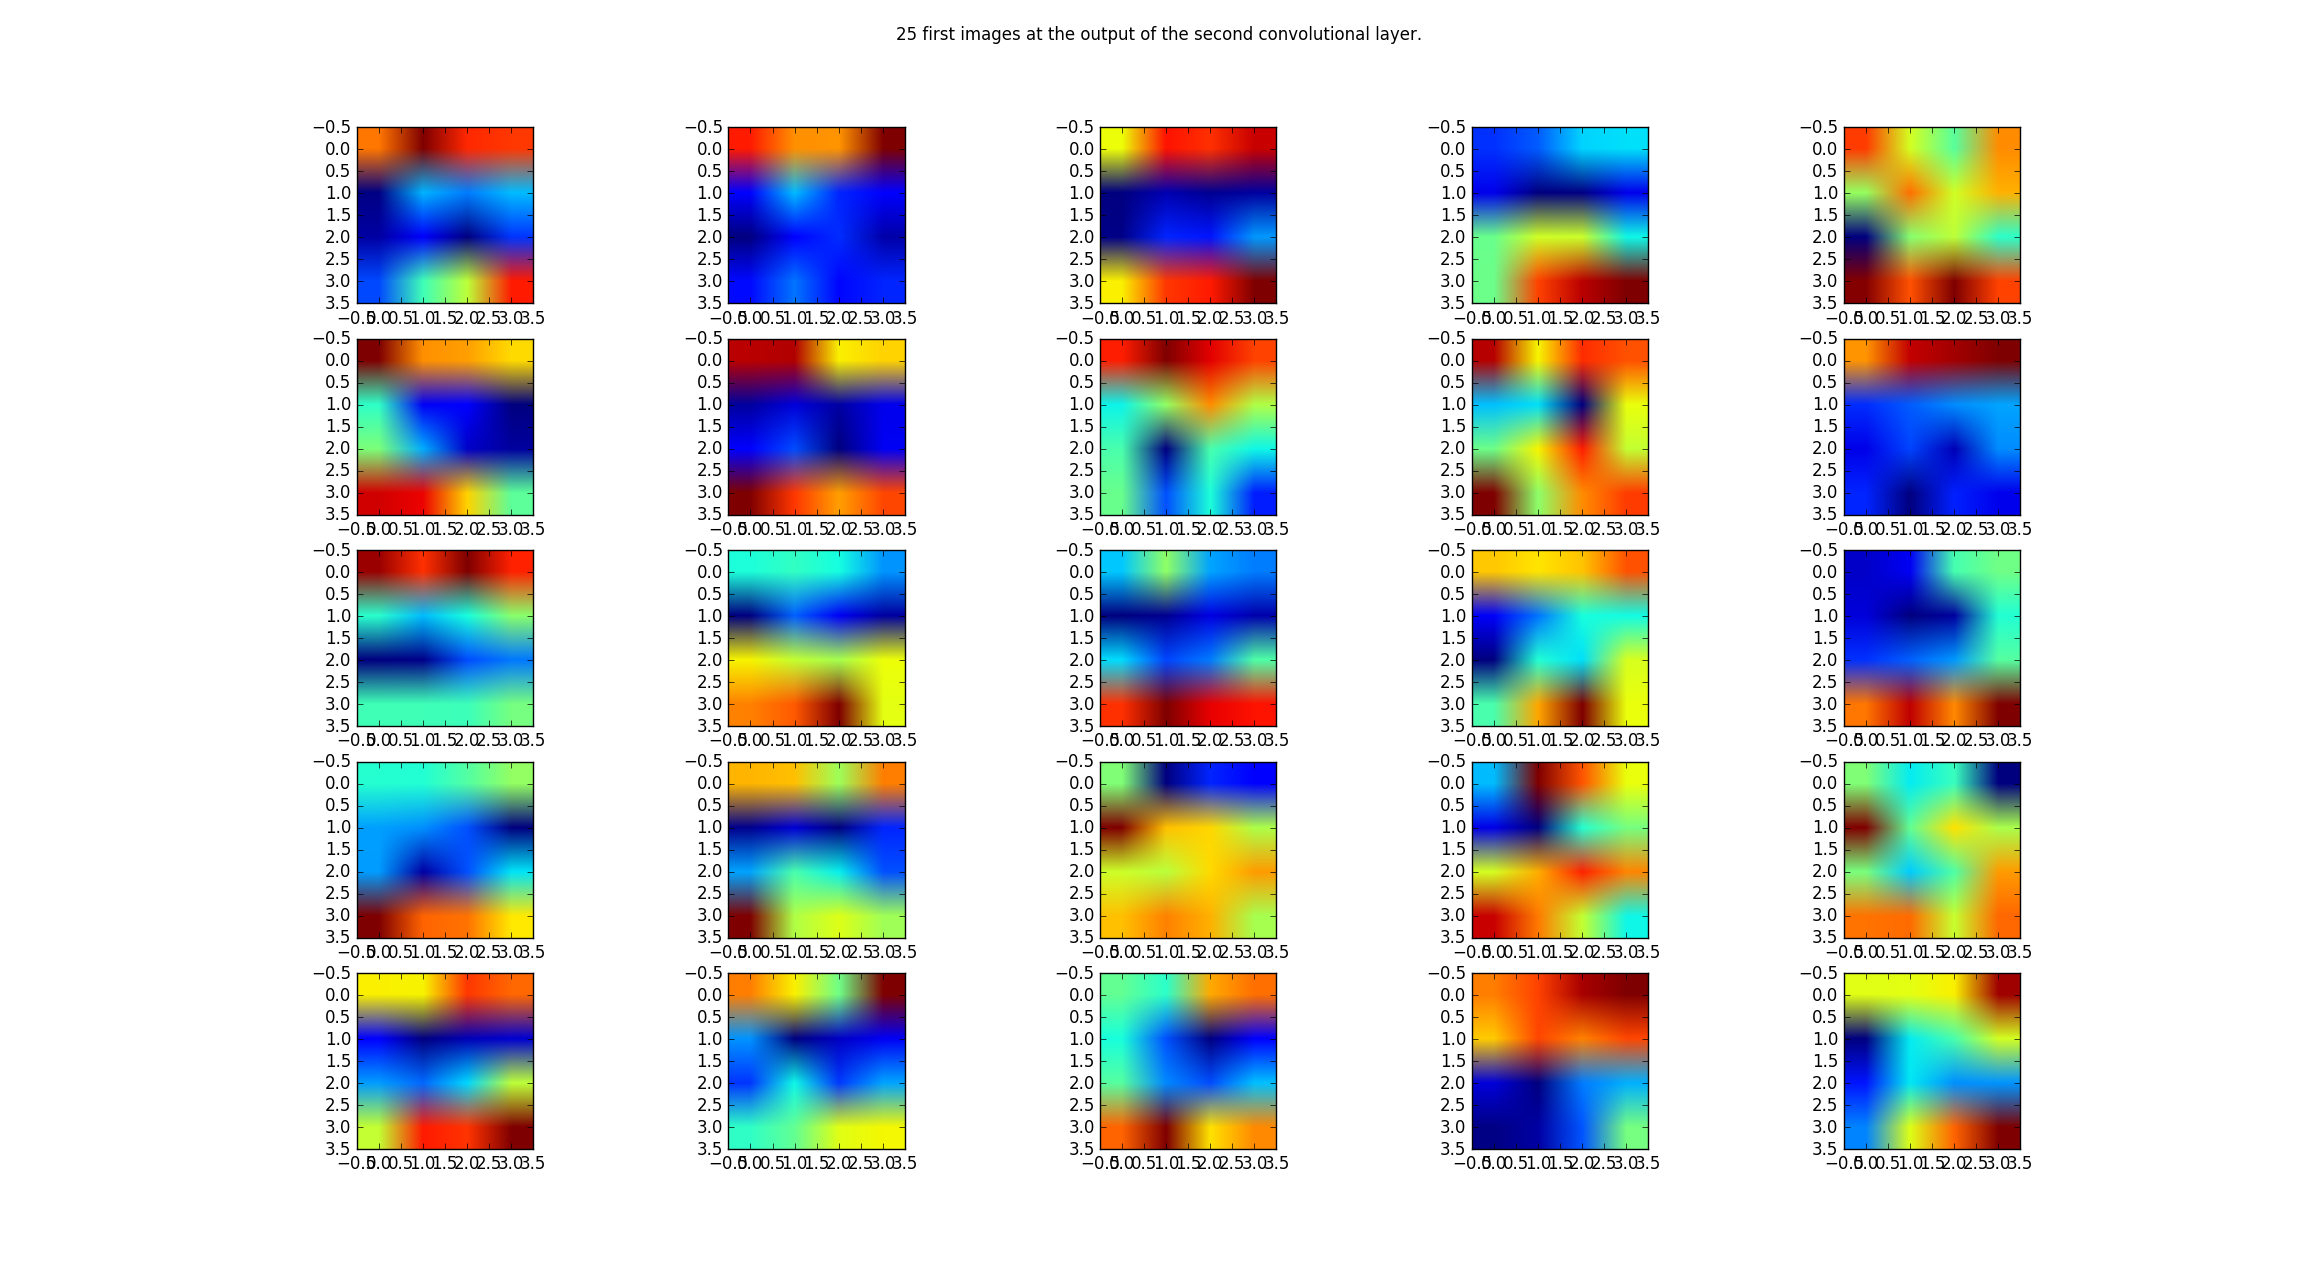
\includegraphics[width=1.4\textwidth]{images/LFW_layers/conv_1_out.png}
\caption{Output of the convolutional layers using LeNet and LFW.} \label{fig:LENETLFW_ker4}
\end{figure}

The result of the third example is a best validation score of 95.73 \% obtained at iteration 546, with test performance 95.23 \%. \\

The cost function of those three experiments are represented in \ref{fig:LENETLFW_Cost}

\begin{figure}[htb]
    \centering
        \subfigure[Example 1]{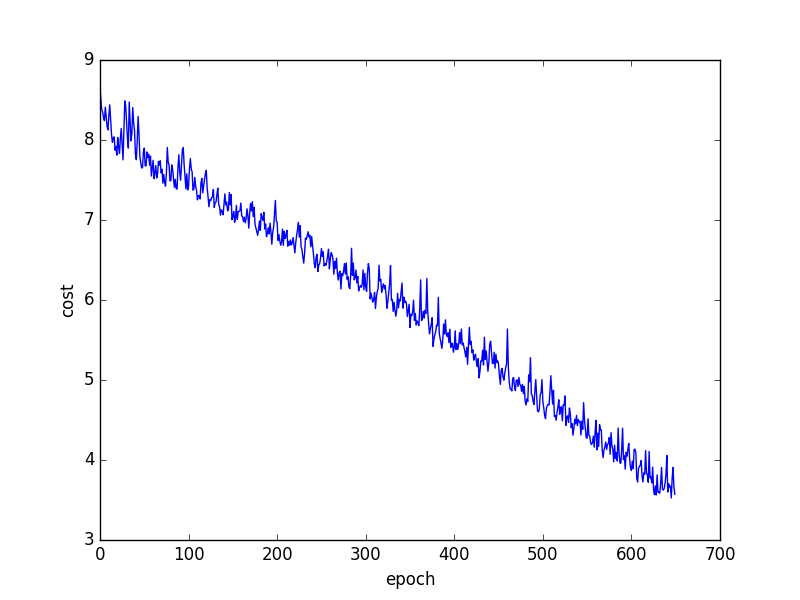
\includegraphics[width=0.47\textwidth]{images/LFW_layers/cost_conv_40_60.png}}
        \subfigure[Example 2]{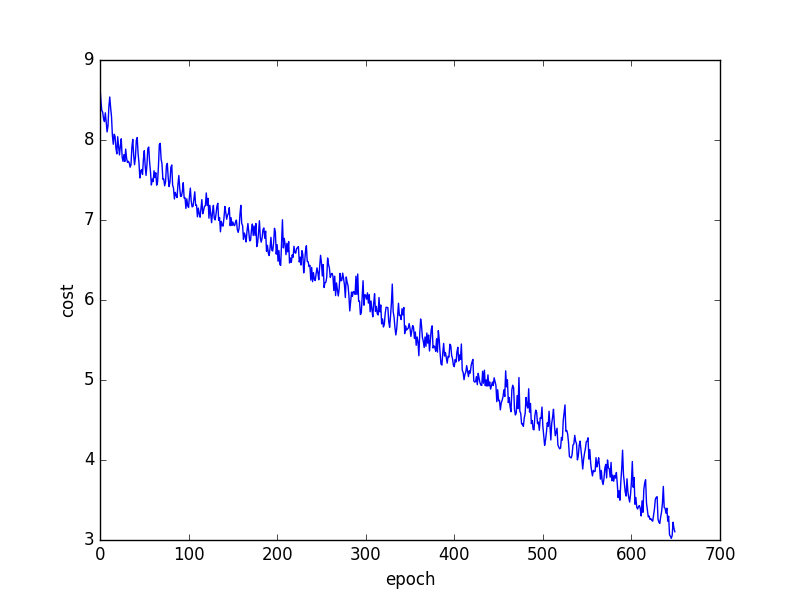
\includegraphics[width=0.47\textwidth]{images/LFW_layers/cost_conv_40_60_2.png}}
		\subfigure[Example 3]{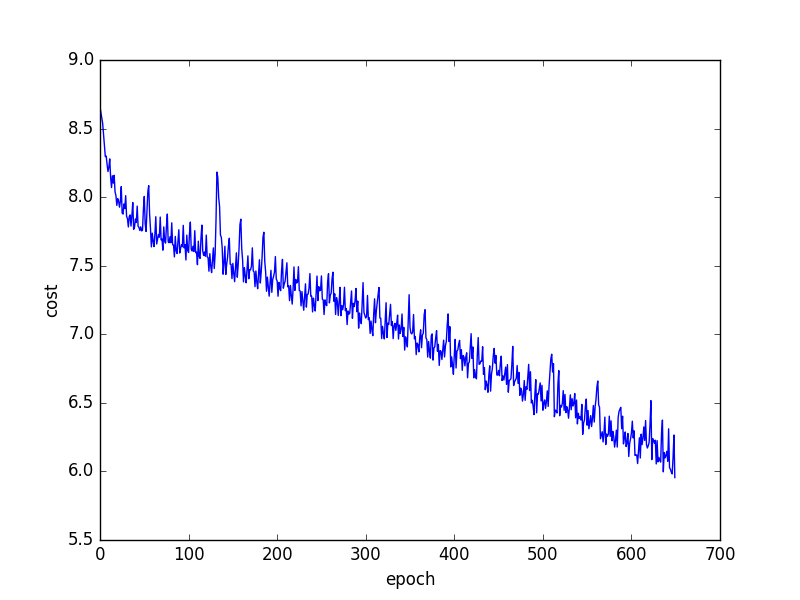
\includegraphics[width=0.47\textwidth]{images/LFW_layers/cost_conv_40_60_3.png}}

    \caption{Cost function at training of the three examples chanching the convolutional parameters.} \label{fig:LENETLFW_Cost}
\end{figure}

%\subsubsection{Changing pooling parameters}
%The theano function used to build this kind of layer depends of theano version,


\subsubsection{Using ReLu as an activation function instead of tanh}
Originally LeNet uses as activation function tanh(), but in this section, ReLu (Rectified linear units) activation function is going to be used. In equation \ref{Relu-formula} is shown how it is defined.  \\

\begin{equation}
f(x) = max(0,x)
\label{Relu-formula}
\end{equation}

The error and the cost in each epoch could be seen in figure \ref{fig:LENET_relu}

\begin{figure}[htb]
\centering
		\subfigure[Cost at training]{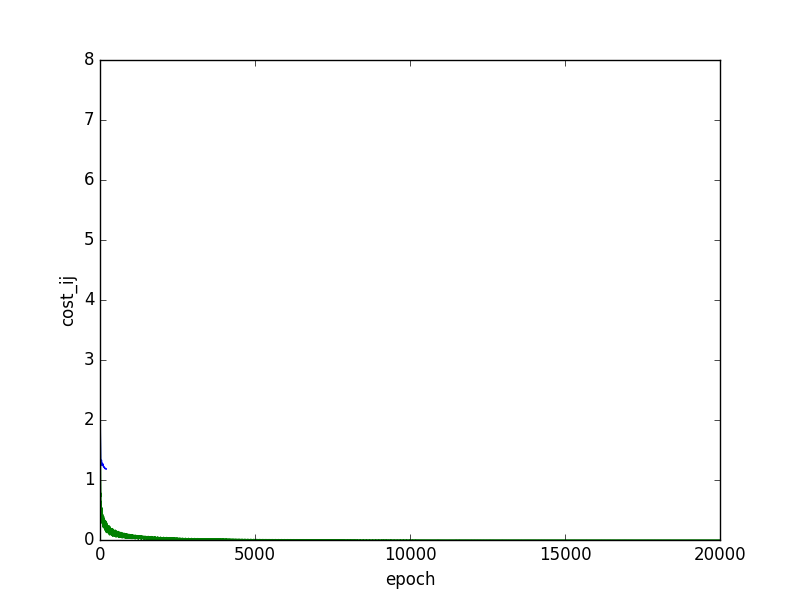
\includegraphics[width=0.47\textwidth]{images/images_lenet/cost_relu.png}}
		\subfigure[Error at validation]{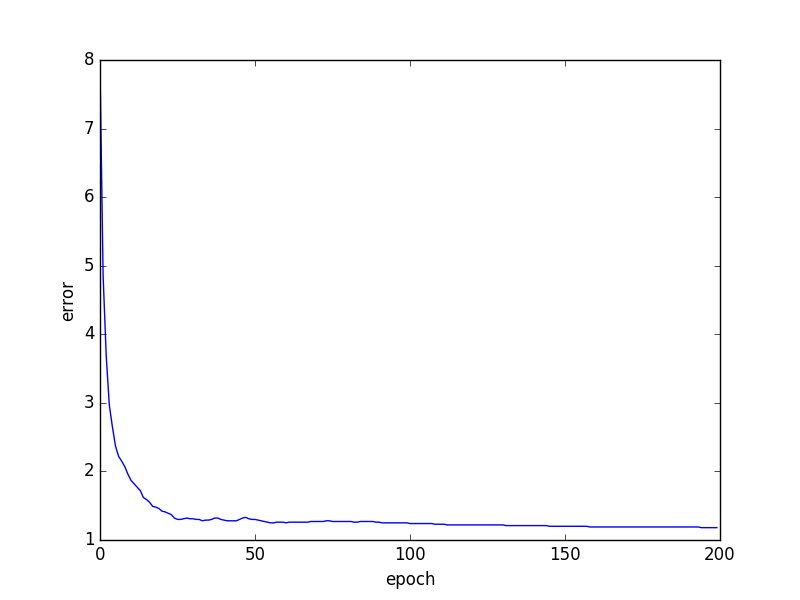
\includegraphics[width=\textwidth]{images/images_lenet/error_relu.png}}

\caption{Error and cost using ReLu instead of tanh}
\label{fig:LENET_relu}
\end{figure}

\subsection{Using FRAV dataset}
One of the databases used with the final architecture and configuration of the network is FRAV database. LeNet-5 is tested with this database in this current section.\\

The experiments made with this database are just with RGB images, so 939 images of people has been used, 489 samples are used for the training subset, 162 samples has been used in the validation subset and 279 samples in the test subset.\\

Because images has not the same shape, they have been re-sized into 252x180, this new shape is proportional 0.7*height = weight because all images studied save that proportion. In addition, making images smaller also gives the security of not having memory problems, because the huge quantity of used images.\\

The network has been tested with this databases in the two ways of classify images, with two classes (genuine and attacks) and five classes (genuine and four classes, one per type of attack).\\ %Also, different learning rates have been used.\\

The first experiment made was based in the neural network LeNet, without changing parameters, but batch size because 500 is too big, there are not enough samples:\\

\begin{itemize}
\item 25 epoch.
\item 20 and 50 kernels of each convolutional layer.
\item 50 batch size.
\item 0.01 learning rate.
\item Logistic regression with 10 neurons.\\
\end{itemize}

The obtained results are with 5 classes classification and there were not as bad as the one with labeled faces in the wild (LFW), in this database there are more samples per class.\\

Figure \ref{fig:FRAV_five} shows the validation error of five classes, the best validation error has token place in epoch 7 with test performance 60.4\%. It has token 68.78 minutes to run.\\

\begin{figure}[htb]
\centering
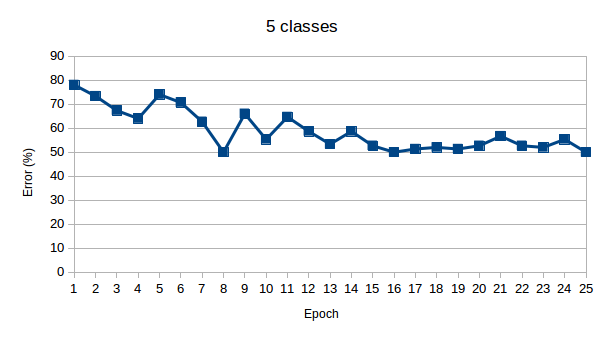
\includegraphics[width=0.7\textwidth]{images/epoch_5classes_FRAV_1.png}
\caption{Error using FRAV database and five classes.}
\label{fig:FRAV_five}
\end{figure}

In figure \ref{fig:FRAV_two}, the validation error in different epoch could be visualized using two classes to classify. It could be seen that in each epoch the validation error is the same. Test error performance at the first epoch is 23.2 \%. The total time of the running has been 64.0167 minutes.\\

\begin{figure}[htb]
\centering
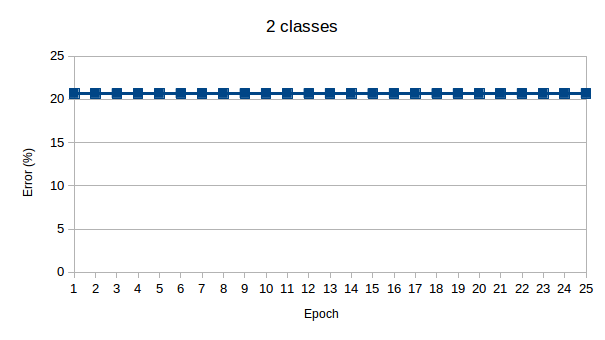
\includegraphics[width=0.7\textwidth]{images/epoch_2classes_FRAV_1.png}
\caption{Error using FRAV database and two classes.}
\label{fig:FRAV_two}
\end{figure}

The time in both cases, classifying with two or five classes are similar, but not the result, is better when just two classes are used and no differentiation is made among attacks. There would be need more samples and more time to get a better score if five classes classification is wanted.\\

% TODO For the time being no differentiation among classes is done, there is no necessity to differentiate the attacks, so the classification is going to be bi-classe: genuine and attack.\\

\section{Defining a new architecture}
From the LeNet-5 code, which is proportioned by \url{deeplearning.net}, changes has been developed to build a new architecture \cite{LSTM-CNN}. \\

%After this, the CNN has been changed in order to build a CNN similar to the one described in \textit{Learning Temporal Features Using LSTM-CNN Architecture for FaceAnti-spoofing}.\\

The new architecture of the Convolutional Neural Network is formed by two convolutional layers, the first one with 48 filters and the second one with 96. The size of the filters is 5x5. Each convolutional layer is followed by a max pool layer of size 2x2.\\

The activation function has been changed to the rectified linear activation function (ReLu), a function implemented in Theano has been used to this purpose \textit{theano.tensor.nnet.relu}. For the weight initialization, a normalized distribution of weights and bias, the same which was implemented in LeNet-5: weights are sampled randomly from a uniform distribution.\\

Because of the huge number of images, the  batch size has been changed to 20. And the learning rate is 0.001. The number of neurons at the output of the hidden layer are 100. The classifier is the sigmoid function. 25 epoch have been used for training the network.\\

the used database in this experiment is Casia database and its samples have been pre-processed, images are resized into 52x104, the relation between width and height is proportional to the original size of images, but they have not the same shape. At the time to split the data into train, test and validation, different seeds have been used with the purpose of test the net with different combination of the data.\\

% NO ENCUENTRO LOS RESULTADOSS
%(AÑADIR LOS RESULTADOS CON LAS DIFERENTES SEMILLAS)

%\subsection{using CASIA dataset}
%Before proving casia databse in the convolutional neural network, the net has been modified in order to diference training and test, so the net train and validate and when a new best score of error is gotten, the network is saved. After training, the best configuration of the network is loaded and tested with the test set.\\

two different ways of using classes has been used, first, two classes has been used, one the imges of the genuine people and another class with the atacks, the last way of separate classes is assigning one different class to a different attack.\\

%Casia database has also been proved using two classes and two seeds.\\

%(AÑADIR LOS RESULTADOS)


\section{Regenerating the databases}
The databases have been generated in a different way from the used before. In this new way, the possibility of access to the misclassified samples is possible. SO the characteristic of misclassified images could be studied. This is not used now, but in the future it could be useful.\\

In order to build the new database, a script as been programmed manually because the test-train split sklearn function does not let know what image has been read and now it is possible to compare the right class of each image with the predicted one.\\

All this work has been changed because it is interesting to know the characteristics of people (if has beard, glasses or long hair) that are not well classified.\\

It has been necessary to shuffle the data twice in order to mix it properly and training, testing and validating test would have data of the five classes.\\

\subsubsection{Adding images in characteristic level}
In order to get this particular goal, each image is re-sized proportionally to original image to 52x104 dimensions. Each NIR image is appended to its correspondent RGB image.\\

In order to create a list of images where images are not putted in order, each image followed by another could be of a different class. Two shuffles has been necessary, the first one with a seed = 0.5 and the second one with a seed = 0.1, so the randomize order of images could be repeated.\\

For training, the 70\% of the total data has been used, for testing the 20\% and for validating the testing 10\%. There are 157 images in each class and the distribution is represented in the table \ref{FRAV_distribution1}.\\

\begin{table}[htb]
\centering
\label{FRAV_distribution1}
\begin{tabular}{c|ccccc|c|}
\cline{2-7}
                                     & \multicolumn{1}{c|}{Class 0} & \multicolumn{1}{c|}{Class 1} & \multicolumn{1}{c|}{Class 2} & \multicolumn{1}{c|}{Class 3} & Class 4 & Total of samples \\ \hline
\multicolumn{1}{|c|}{Training set}  & 94                           & 119                          & 116                          & 145                          & 76      & 550              \\ \cline{1-1}
\multicolumn{1}{|c|}{Testing set}    & 33                           & 38                           & 37                           & 7                            & 42      & 157              \\ \cline{1-1}
\multicolumn{1}{|c|}{Validating set} & 30                           & 0                            & 4                            & 5                            & 39      & 78               \\ \hline
\end{tabular} \caption{Distribution of samples FRAV (RGB + NIR) database}

\end{table}

The code runs for 150 epoch with a learning rate of 0.001 and a batch size of 20 images.\\

The disadvantage of using mini-batches is that there are some images remain and the quantity os less than a mini-batch, that images are not used, so from 157 testing images, just 140 has been used.\\

The test error that has been gotten is 30\% at iteration 1863 where the best validation score was gotten (26,67\%). Where:

\begin{itemize}
\item Class 0 has been misclassified  14 times
\item Class 1 has been misclassified  6 times
\item Class 2 has been misclassified  7 times
\item Class 3 has been misclassified  2 times
\item Class 4 has been misclassified  2 times
\end{itemize}

To get that results 3,04 hours was needed to run the code.\\

%y_pred = [2,4,2,1,2,1,2,1,4,0,3,1,2,1,2,0,2,0,3,1,3,1,3,1,2,1,2,1,4,1,2,4,2,1,2,1,2,1,2,1,2,1,3,1,2,1,2,0,2,1,2,1,3,1,2,1,2,1,3,1,4,1,2,1,2,1,2,1,3,1,2,1,2,1,2,1,0,4,3,4,0,1,1,4,1,4,1,4,2,4,0,4,1,4,0,4,1,4,2,4,1,4,1,1,0,4,0,4,2,4,0,4,1,4,0,4,0,4,3,4,4,4,0,4,1,4,4,4,2,4,0,4,1,4,1,4,1,4,3,4]

%y_real = [2,1,2,1,2,1,2,1,4,1,2,1,2,1,2,1,2,1,3,1,2,1,2,1,2,1,2,1,4,1,2,1,2,1,2,1,2,1,3,1,2,1,2,1,2,1,2,1,2,1,2,1,2,1,2,1,2,1,3,1,2,1,2,1,2,1,2,1,2,1,2,1,2,1,2,1,0,4,3,4,0,4,0,4,0,4,0,4,2,4,0,4,0,4,0,4,0,4,3,4,0,4,0,4,0,4,0,4,2,4,0,4,0,4,0,4,0,4,3,4,0,4,0,4,0,4,0,4,2,4,0,4,0,4,0,4,0,4,3,4,0,4,0,4,0,4,0,4,2,4,0,4,0,4,0,4,0]


%\section{Metrics}
%In order to measure the net and its works, some metrics would be used, but %to do that, the data has to be splited in other way because with the %function train\_test\_split there is no chance, which is know, to get the %image if it is not printed; so a own method has been developed and it is %posible too pseudo-randomize the data.\\

%The metrics that has been used are:
%\begin{itemize}
%\item FAR: False aceptance rate
%\item FRR: False rejection rate
%\end{itemize}

\clearpage

\subsection{Architecture implemented in Casia videos}
In this section, the architecture used in the paper of the Casia videos would be repeated partially. The paper is learn convolutional neural network for face anti-spoofing.\\

The architecture followed in the paper is the same used in Imagenet, it is formed by five convolutional layers, followed by three fully-connected layers. The two first conv layer and the last one are followed by a max-pool layer. The two first conv layers are followed by response normalization layers too. Authors use ReLu like activation function in each layer. The first two fully-connected layers are followed by two dropout layers, and the last layer output is followed by softmax layer as a classifier.\\

Authors do not explain anything else about the architecture. In the paper of Imagenet is said that:

\begin{itemize}
\item The ReLU non-linearity is applied to the output of every convolutional and fully-connected layer.
\item The first convolutional layer filters the 224×224×3 input image with 96 kernels of size 11×11×3 with a stride of 4 pixels.
\item The second convolutional layer takes as input the (response-normalized and pooled) output of the first convolutional layer and filters it with 256 kernels of size 5 × 5 × 48.
\item The third, fourth, and fifth convolutional layers are connected to one another without any intervening pooling or normalization layers.
\item The third convolutional layer has 384 kernels of size 3 × 3 × 256 connected to the (normalized, pooled) outputs of the second convolutional layer.
\item The fourth convolutional layer has 384 kernels of size 3 × 3 × 192.
\item  The fifth convolutional layer has 256 kernels of size 3 × 3 × 192.
\item The fully-connected layers have 4096 neurons each.
\item The maxpool size filter si 2x3 because it reduces the error 0.4\% - 0.6\% compared to 2x2 filters.
\item In Imagenet uses 224x224 images.
\end{itemize}

It is not explained how authors change the architecture of Imagenet.\\

The data used to this experiment is the Casia database, the one that uses in the paper, although authors, use Reply-attack too.\\

The data is composed by two folders, a training folder and a test data, in each folder there are some user folders, in each user folders there are two videos from the real user, tho videos of the user with a mask, two videos with the mask and with a hole in the eyes and two videos with a digital screen where a user is shown in the screen. 3 attacks are presented, so four classes are used (real users, users with mask, users with mask and eyes and a digital screen). It is not specified how many frames authors use, so it s supposed that they use all the video.\\

For each frame, the face is looked for in the image with viola jones algorithm implemented in opencv, and the image is cropped and saved, but in that image cropped there is no background, so different scales, 1.4, 1.8, 2.2, 2.6, are used to get background, because in learn convolutional neural network for face anti-spoofing and then images are re-sized to 128x128.\\

In order to carry out this experiment, a better computer has been needed because it was no possible to run with the same that the utilized in the previous experiments.\\

But with a better computer, it is not possible read more than 2 or 3 frames per video to run the net, because it has a huge architecture with a big quantity of filters per layer.\\

So the experiment with the videos has not been possible to be carried out.\\

In addition, is it not possible to carry out the architecture of imagenet with the size of Casia images because if it is started with 128x128 images, at the end,  images sizes are images of < 1px.\\

In order to know how strides work, a python file has been created called understanding strides, in which a pickle format file is loaded. This pickle format file is the output of a layer, and it is possible to see the size of images of the layer. So it is possible to know the size of images after striding and this number could be saved to be written in the conv layer.\\

In this computer, the theano function used to build the max\-pool layer has changed bacuse of Theano version, the previous function used in Theano  \textit{theano.te\-nsor.sig\-nal.down\-sam\-ple.max\-\_pool\_2d} has been replaced by \textit{thea\-no.ten\-sor.sig\-nal.pool.pool\_2d} using the mode \textit{max}.\\

To  sum up, In this first experiment, the architecture is formed by the convolutional and pooled out layers but without strides. The folder where this experiment has been developed has been in frav\_casia\_imagenet. The architecture is just based in conv, pool and hidden layer (no dropout, softmax or normalization layer). In figure \ref{fig:error_imagenet1} it is possible to see how the error is descending in each epoch and get stabilized with a 5\% aprox. error. \\
\begin{figure}[htb]
\centering
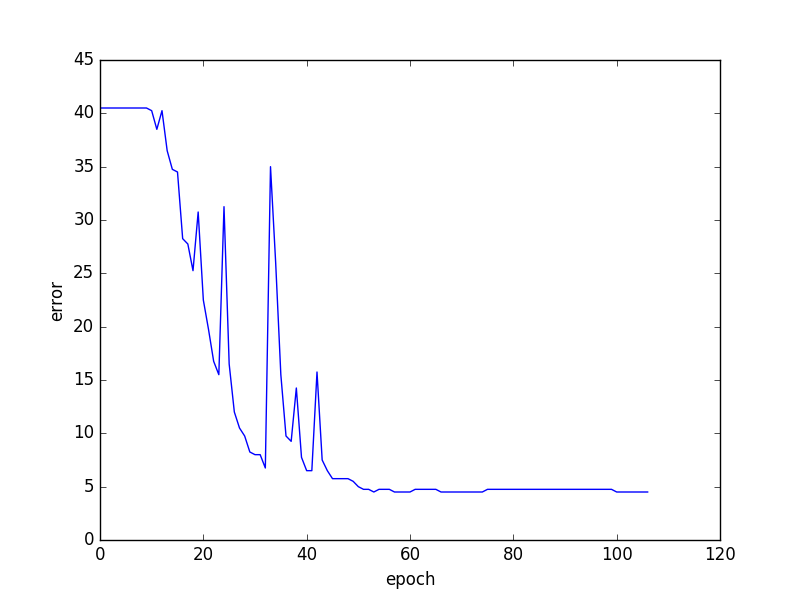
\includegraphics[width=0.7\textwidth]{images/imagenet/error_frav-Imagenet1.png}
\caption{Error of Lenet in the first try to build imagenet.} \label{fig:error_imagenet1}
\end{figure}

The code had been running for 364,39 hours. And the true positive rate, true negative rate, false positive rate and false negative rate are available in table \ref{tabla_error_imagenet1}. \\

\begin{table}[htb]
\centering
\label{tabla_error_imagenet1}
\begin{tabular}{lllll}
\cline{1-4}
\multicolumn{1}{|l}{TP} & \multicolumn{1}{l}{TN} & \multicolumn{1}{l}{FP} & \multicolumn{1}{l|}{FN} &  \\ \cline{1-4}
\multicolumn{1}{|l}{156} & \multicolumn{1}{l}{623} & \multicolumn{1}{l}{10} & \multicolumn{1}{l|}{11} &  \\ \cline{1-4}
                         &                         &                         &                         &  \\
                         &                         &                         &                         &
\end{tabular}
\caption{TP, TN, FP, FN rates in the first trying of imagenet.}

\end{table}

\clearpage
%\subsection{Reading frav faces}
%He hecho un base de datos generator, en el que voy creando la base de datos, dentro de esa carpeta hay un info en el que se explica como se leen las imagenes. Puedes escalarlas, puedes buscar caras o no y en guardarlas en distintas escalas como en casia.\\


\subsection{As close as possible as Imagenet}
%Dentro de la carpeta de FRAv\_casia\_ImageNet, en imagenet2, se ha programado imagenet, lo unico que sin strides en la primera capa de convolucion.\\
Because of the lack of information about the convolutional neural network described in casia paper, it has been necessary  to though the original code that authors use, Imagenet. Authors use the same architecture, although how it has been modified it is not explained. \\

It has been possible to implement Imagenet, the difference between the implementation and the original one is that the strides used in the first convolutional layer has not been used because the input of the images need to be bigger to have more than one neuron in the last layer.\\

%Dentro hay una carpeta para cada base de datos. Dentro de cada carpeta estan las pruebas que se hacen con cada base de datos.\\

The convolutional neural network has been tested with different databases: FRAV, CASIA and MFSD and different experiments have been carried out with each one.\\

\subsubsection{Network configuration for each experiment}
The configuration of each experiment of each network are described in the following lines. When it is said that Gaussian weight initialization has been used, the mean value is 0 and the std used is 0.01 in all the times ans bias has been initialized to 1, if not, bias has been initialized to 0. When Gaussian initialization has not been used,  weights are sampled randomly from a uniform distribution in the range [-1/fan-in, 1/fan-in], where fan-in is the number of inputs to a hidden unit [copy-paste from deeplearning.net]. \\

The goal of the next experiments is getting an optimal architecture changing the parameters. the difference between using a normal distribution o a Gaussian distribution of weights initialization has been tested and using SVM with linear kernel and RBF kernel has been tried.\\

FRAV database (Common parameters:  n\_epochs=400, nkerns=[96, 256, 386, 384, 256], batch\_size=20):\\
\begin{itemize}
\item frav1: Gaussian weights initialization. SOFTMAX used as classifier. Learning rate = 0.001 Figure \ref{fig:Imagenet2-frav1}.
\item  frav\_gaussian\_initinizialization: Gaussian weight Initialization. Learning rate = 0.001. SOFMTAX used as classifier. Figure \ref{fig:Imagenet2-frav_gaussian_init} .
\item svm\_gauss: Using SVM (with RBF kernel) as classifier. Gaussian weight Initialization. Learning rate = 0.01 \ref{fig:Imagenet2-frav-svm_gauss}.
\item svm\_genera: Using as a classifier SVM with RBF kernel. Learning rate = 0.01 \ref{fig:Imagenet2-mfsd-svm_general}.
\item svm\_linear: Classifying with SVM (linear) and Gaussian weight initialization. Learning rate = 0.01\\
\end{itemize}

CASIA (images) ( nkerns=[96, 256, 386, 384, 256]):\\
First, four test has been carries out (in which the learning rate has been changed and the number of epochs. trying to get the best learning rate configuration. In four test the batch size used is 25 samples, the classifier used at testing is Softmax and the weight initialization used is normal distribution.:\\
\begin{itemize}
\item Test1: learning\_rate=0.01, nepochs=400.
\item Test2: learning\_rate=0.001, n\_epochs=400.
\item Test3: learning\_rate=0.0005, n\_epochs=400.
\item TEst4: learning\_rate=0.001, n\_epochs=1000,
\end{itemize}

It has not been possible getting a train loss that converge in a minimum in none of the four tests. A good train loss should decrease in each epoch until converge in a minimum. But in the tests, the
- casia\_gaussian\_init: gausiana de pesos con mean 0 y std 0.01. SOFMTAX como clasificador. learning\_rate=0.01, n\_epochs=400, nkerns=[96, 256, 386, 384, 256], batch\_size=20 \\
- svm\_gauss: Utilizando svm (rbf) como clasificador, con inizializacion normal. learning\_rate=0.01, n\_epochs=400, nkerns=[96, 256, 386, 384, 256], batch\_size=20\\
- svm\_general: utilizando SVM (rbf) con inicializacion de pesos gaussiana. learning\_rate=0.01, n\_epochs=400, nkerns=[96, 256, 386, 384, 256], batch\_size=20\\
- svm\_linear: SVM (linear) con inicializacion de pesos gaussiana. learning\_rate=0.01, n\_epochs=400, nkerns=[96, 256, 386, 384, 256], batch\_size=20\\

MFSD  (learning\_rate=0.01, n\_epochs=400, nkerns=[96, 256, 386, 384, 256], batch\_size=20):\\
- svm\_gauss: Utilizando svm (rbf) como clasificador, con inizializacion gaussianana.\\
- svm\_genera:utilizando SVM (rbf) con inicializacion de pesos gaussiana \\
- svm\_linear: SVM (linear) con inicializacion de pesos gaussiana\\

IMPORTANT: The valid graphs are made with SOFTMAX independly of the classifier used to test.\\

\subsubsection{Results with FRAV database}

In this section, cost (at training) and error (at validating) is going to be visualized. First when FRAV database has been trained with Gaussian initialization and with a learning rate = 0.001 \ref{fig:Imagenet2-frav1}. Second with the same learning rate, but Gaussian initialization for weights \ref{fig:Imagenet2-frav_gaussian_init}. Third, decreasing the learning rate to 0.01 and with normal initialization \ref{fig:Imagenet2-frav-svm_general} and the last one, whit the same learning rate but with Gaussian weights initialization \ref{fig:Imagenet2-frav-svm_gauss}.\\


\begin{figure}[htb]
\centering
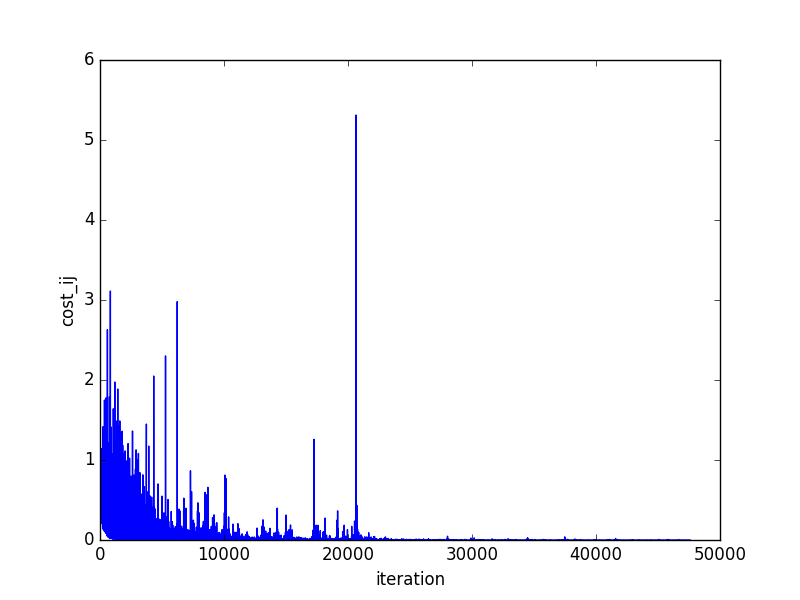
\includegraphics[width=0.45\textwidth]{images/FRAv_casia_ImageNet/Imagenet2/frav/frav1/cost_frav.png}
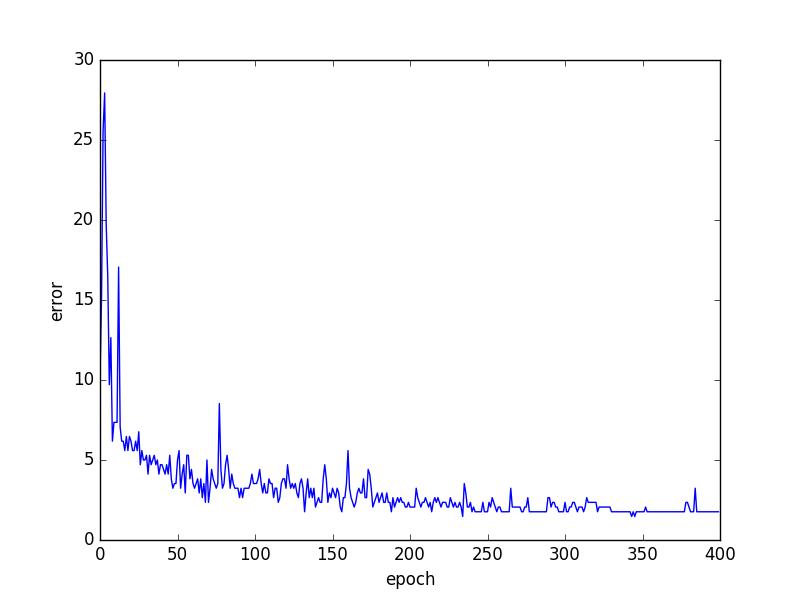
\includegraphics[width=0.45\textwidth]{images/FRAv_casia_ImageNet/Imagenet2/frav/frav1/error_frav.png}
\caption{Cost at training and error at validating. Normal initialition. Learning rate = 0.001 (frav1).} \label{fig:Imagenet2-frav1}
\end{figure}

\begin{figure}[htb]
\centering
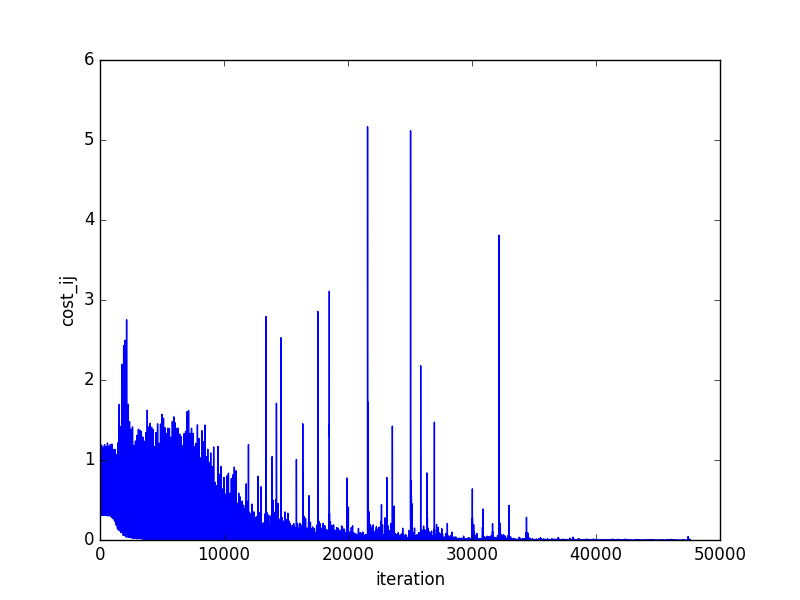
\includegraphics[width=0.45\textwidth]{images/FRAv_casia_ImageNet/Imagenet2/frav/frav_gaussian_init/cost_frav.png}
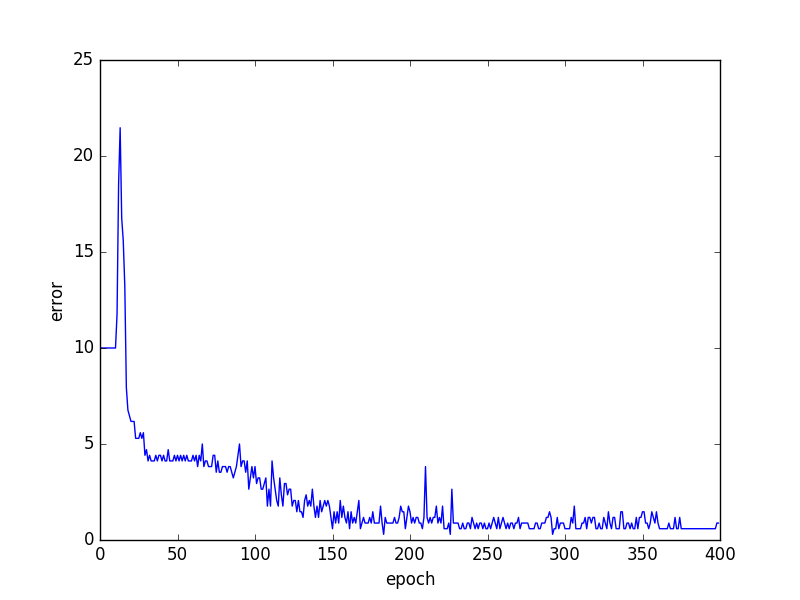
\includegraphics[width=0.45\textwidth]{images/FRAv_casia_ImageNet/Imagenet2/frav/frav_gaussian_init/error_frav.png}
\caption{Cost at training and error at validating. Gassian initialization. Learning rate = 0.001 - frav\_gaussian\_init} \label{fig:Imagenet2-frav_gaussian_init}
\end{figure}

\begin{figure}[htb]
\centering
\includegraphics[width=0.45\textwidth]{images/FRAv_casia_ImageNet/Imagenet2/frav/svm_gauss/cost.png}
\includegraphics[width=0.45\textwidth]{images/FRAv_casia_ImageNet/Imagenet2/frav/svm_gauss/error.png}
\caption{Cost at training and error at validating - Gaussian initialization. learning rate = 0.01 frav svm\_gauss.} \label{fig:Imagenet2-frav-svm_gauss}
\end{figure}

\begin{figure}[htb]
\centering
\includegraphics[width=0.45\textwidth]{images/FRAv_casia_ImageNet/Imagenet2/frav/svm_general/cost.png}
\includegraphics[width=0.45\textwidth]{images/FRAv_casia_ImageNet/Imagenet2/frav/svm_general/error.png}
\caption{Cost at training and error at validating - Noraml initialization. learning rate = 0.01 frav svm\_general.} \label{fig:Imagenet2-frav-svm_general}
\end{figure}


First FRAV experiment (SOFTMAX as classifier and regular initialization) gives good results. The cost converges to 0 at training, the validation gets a 1.470588 \% best error rate with test performance of 5 \%. In testing, just 10 samples has been misclassified (7 samples of class 0 and 3 of class 1, from 679 test samples as total. The ROC  and precision-recall curves could been visualized figure \ref{fig:Imagenet2-frav-frav1ROC}\\

\begin{figure}[htb]
\centering
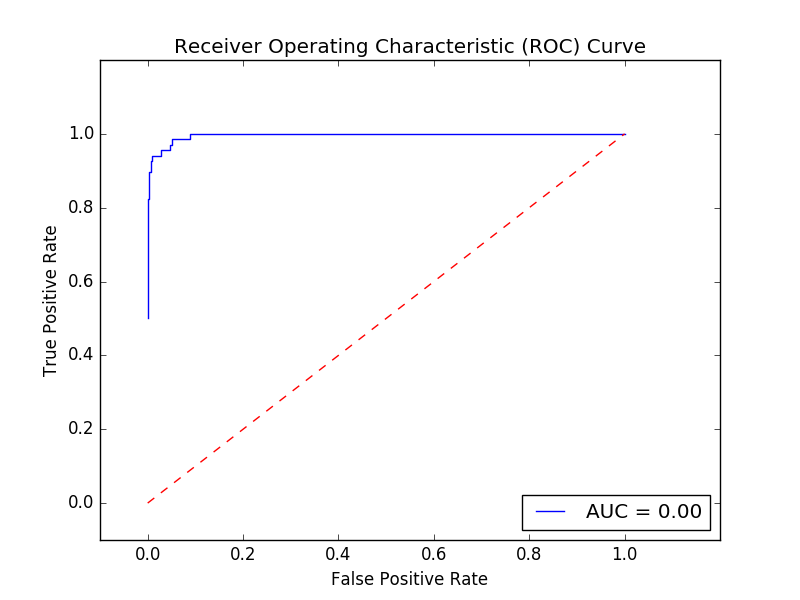
\includegraphics[width=0.45\textwidth]{images/FRAv_casia_ImageNet/Imagenet2/frav/frav1/ROC.png}
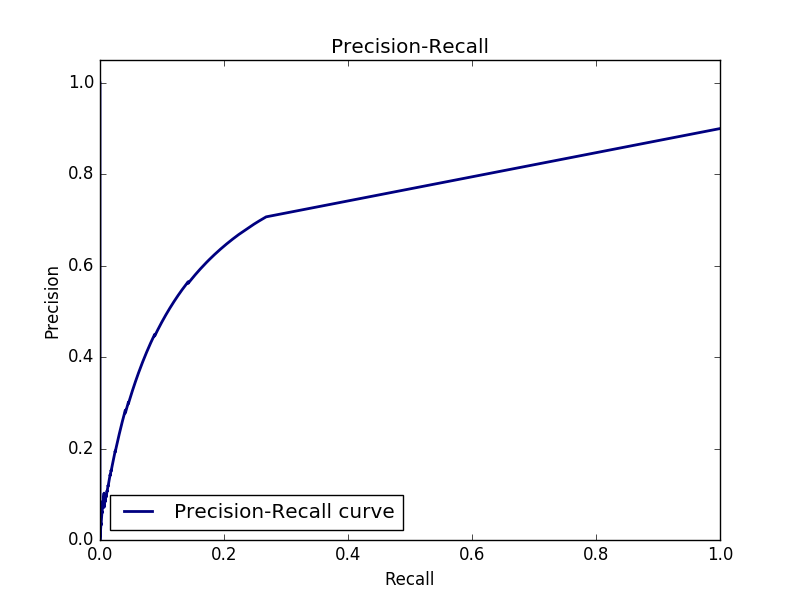
\includegraphics[width=0.45\textwidth]{images/FRAv_casia_ImageNet/Imagenet2/frav/svm_general/Precision-Recall.png}
\caption{ROC and Precision- Recall courve - Noraml initialization. learning rate = 0.01 frav svm\_general.} \label{fig:Imagenet2-frav-frav1ROC}
\end{figure}

It could be seen in the graphics that the Gaussian initialization does not matter when the learning rate is 0.01, but the cost changes when the learning rate is 0.001. In this case, the learning rate 0.001 should be the chosen one.\\

In the table \ref{fravv} The positive and negative rates are visualized from the different classifier (softmax and SVM) the two different weights initialization and the two learning rates used. The results of the table are the same when the learning rate is 0.01 independently of the weight initialization or the kernel used to classify. The metrics rate are not too bad, with the learning rate the results are worse, the learning rate is too big.\\

\begin{table}[htb]
\centering
\begin{tabular}{|ccccccc|}
\hline
Classifier &  Weight initialization & learning rate & TP  & TN  & FP  & FN \\ \hline
Softmax    &         Normal        &     0.001     & 61  & 609 &  3  & 7  \\
Softmax    &       Gaussian        &     0.001     & 66  & 605 &  7  & 2   \\
SVM RBF(C=5)&         Normal       &     0.01      & 63  & 593 & 19  & 5  \\
SVM RBF(C=5)&         Gaussian     &     0.01      &  63 & 593 & 19  &5  \\
SVM lineal(C=5)&      Gaussian     &     0.01      &  63 & 593 & 19  &5  \\
\hline
\end{tabular} \label{fravv}

\end{table}


\subsubsection{casia results}
For Casia, different experiments has been carried out in order to train the network, using SOFTMAX as classifier and normal weight initialization:\\

\begin{itemize}
\item{Test 1}: Learning rate = 0.01 y 400 epoch.
\item{Test 2}: Learning rate = 0.001 y 400 epoch.
\item{Test 3}: Learning rate = 0.0005 y 400 epoch.
\item{Test 4}: Learning rate = 0.001 y 1000 epoch.
\end{itemize}


In figure \ref{fig:lossCasia4Test} the cost at training could be visualized. In general, should decrease varying its value but decreasing logarithmically. In the first experiment (test 1), the value varies but in a small range, and in general it is constant, in the other three experiments, the cost decreases and this is what must happen, but in test 2 the loss converges two times, after converge the first time, then it increase again ans converges again.\\

In figure \ref{fig:errorCasia4Test} it is possible to see that the error changes but not in a logarithmically way. It increase and decreases its value in each epoch but it all experiments it gets in a 42\% or 40\% error. The desired curve should be as the loss one, but the error should not decrease as much as the training loss does.\\


\begin{figure}[htb]
\centering
		\subfigure[Test 1]{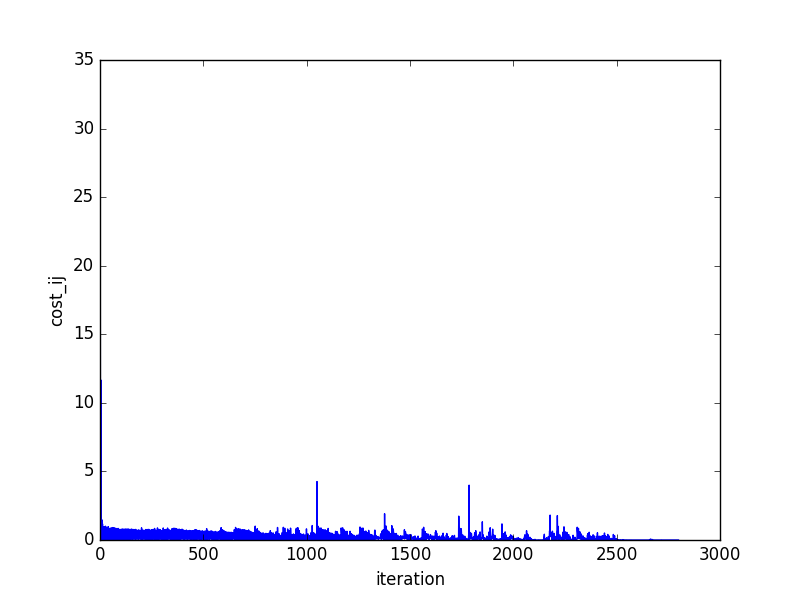
\includegraphics[width=0.47\textwidth]{images/FRAv_casia_ImageNet/Imagenet2/casia/prueba1/cost_frav_p1.png}}
		\subfigure[Test 2]{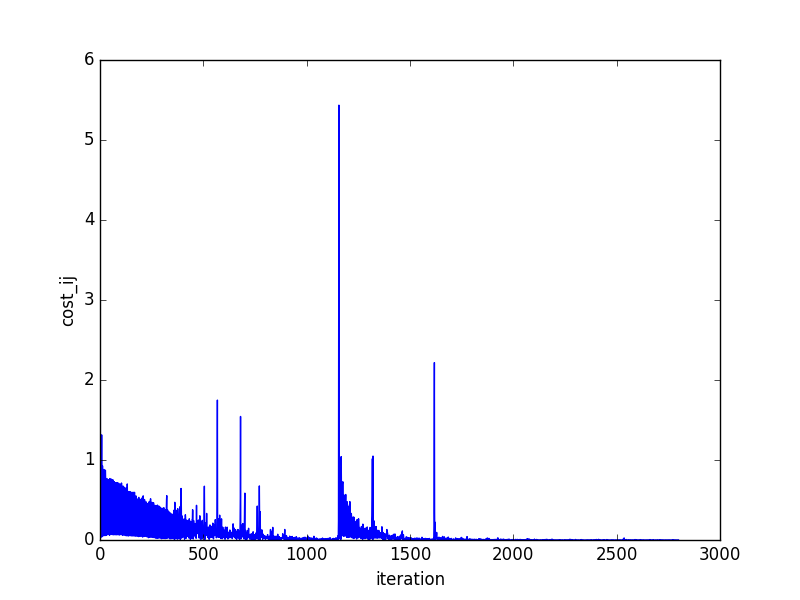
\includegraphics[width=0.47\textwidth]{images/FRAv_casia_ImageNet/Imagenet2/casia/prueba2/cost_frav_p2.png}}			\subfigure[Test 3]{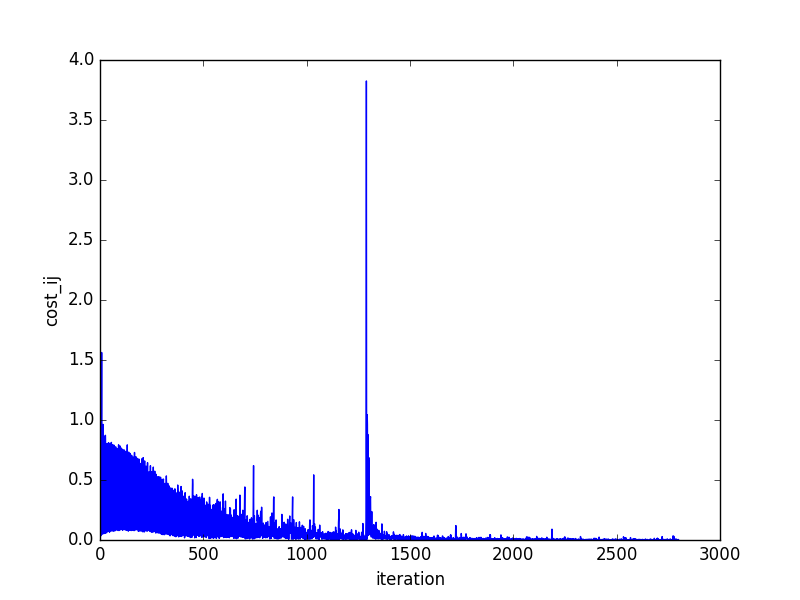
\includegraphics[width=0.47\textwidth]{images/FRAv_casia_ImageNet/Imagenet2/casia/prueba3/cost_frav_p3.png}}
		\subfigure[Test 4]{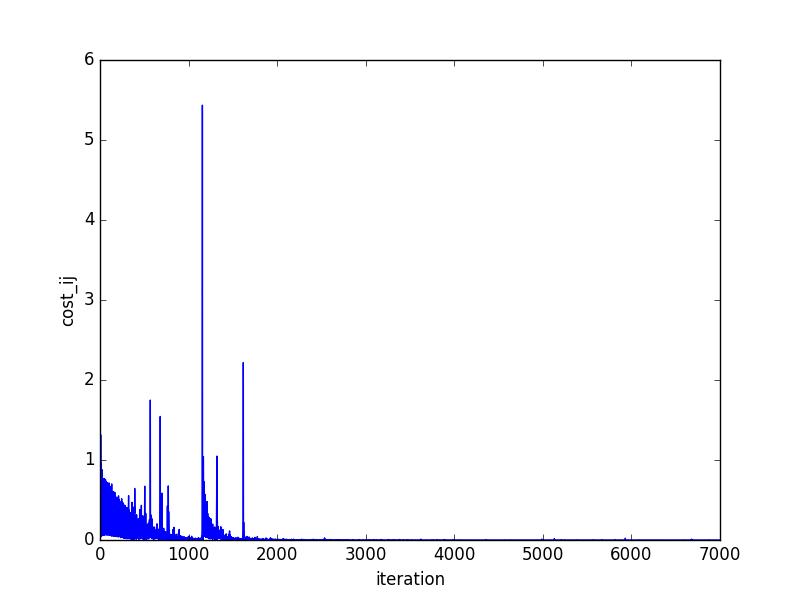
\includegraphics[width=0.47\textwidth]{images/FRAv_casia_ImageNet/Imagenet2/casia/prueba4/cost_frav_p4.png}}
\caption{Training loss of four test Casia database}
\label{fig:lossCasia4Test}
\end{figure}

\begin{figure}[htb]
\centering
		\subfigure[Test 1]{\includegraphics[width=0.47\textwidth]{images/FRAv_casia_ImageNet/Imagenet2/casia/prueba1/error_frav_p1.png}}
		\subfigure[Test 2]{\includegraphics[width=0.47\textwidth]{images/FRAv_casia_ImageNet/Imagenet2/casia/prueba2/error_frav_p2.png}}
		\subfigure[Test 3]{\includegraphics[width=0.47\textwidth]{images/FRAv_casia_ImageNet/Imagenet2/casia/prueba3/error_frav_p3.png}}
		\subfigure[Test 4]{\includegraphics[width=0.47\textwidth]{images/FRAv_casia_ImageNet/Imagenet2/casia/prueba4/error_frav_p4.png}}
\caption{Validation error of four test Casia database}
\label{fig:errorCasia4Test}
\end{figure}


As the same way that in the first experiment that FRAV database converges is that would be expected from Casia, but it has not gotten.\\

\clearpage
At the same way as FRAV, the classifier and the weight initialization has been changed in order to know how the networks behavior with these changes. The learning rate used for this experiment is 0.01. First, the cost (at training) and the error (at validating) are going to be visualized when the weight initialization is normal \ref{fig:Imagenet2-casia-svm_general}. Second when the weight initialization used is Gaussian \ref{fig:Imagenet2-casia-svm_gauss}.\\

%\begin{figure}[htb]
%\centering
%\includegraphics[width=0.45\textwidth]{images/FRAv_casia_ImageNet/Imagenet2/frav/%casia_gaussian_init/cost_frav.png}
%\includegraphics[width=0.45\textwidth]{images/FRAv_casia_ImageNet/Imagenet2/frav/%casia_gaussian_init/error_frav.png}
%\caption{Cost at training and error at testing - casia\_gaussian\_init} %\label{fig:Imagenet2-casia_gaussian_init}
%\end{figure}

\begin{figure}[htb]
\centering
\includegraphics[width=0.45\textwidth]{images/FRAv_casia_ImageNet/Imagenet2/casia/svm_gauss/cost.png}
\includegraphics[width=0.45\textwidth]{images/FRAv_casia_ImageNet/Imagenet2/casia/svm_gauss/error.png}
\caption{Cost at training and error at validating -casia svm\_gauss.} \label{fig:Imagenet2-casia-svm_gauss}
\end{figure}

\begin{figure}[htb]
\centering
\includegraphics[width=0.45\textwidth]{images/FRAv_casia_ImageNet/Imagenet2/casia/svm_general/cost.png}
\includegraphics[width=0.45\textwidth]{images/FRAv_casia_ImageNet/Imagenet2/casia/svm_general/error.png}
\caption{Cost at training and error at validating -casia svm\_general.} \label{fig:Imagenet2-casia-svm_general}
\end{figure}

As the same way than in FRAV database, the cost and at training the error at validating has not changed. The positive and negative rates are the following ones in the three experiments:  TP = 8; TN = 21; FP = 3; FN = 8.\\


\clearpage
\subsubsection{MFSD results}

%\begin{figure}[htb]
%\centering
%\includegraphics[width=0.45\textwidth]{images/FRAv_casia_ImageNet/Imagenet2/mfsd/mfsd_gaussian_init/cost_frav.png}
%\includegraphics[width=0.45\textwidth]{images/FRAv_casia_ImageNet/Imagenet2/mfsd/mfsd_gaussian_init/error_frav.png}
%\caption{Cost at training and error at testing - mfsd\_gaussian\_init} %\label{fig:Imagenet2-mfsd_gaussian_init}
%\end{figure}

As the same way in FRAV and CASIA, but now with MFSD, it is going to be tested the network with a learning rate of 0.01, Gaussian initialization \ref{fig:Imagenet2-mfsd-svm_gauss} and normal distribution initialization \ref{fig:Imagenet2-mfsd-svm_general} and classifying the test with SVM (RBF kernel and linear) and softmax.\\

\begin{figure}[htb]
\centering
\includegraphics[width=0.45\textwidth]{images/FRAv_casia_ImageNet/Imagenet2/mfsd/svm_gauss/cost.png}
\includegraphics[width=0.45\textwidth]{images/FRAv_casia_ImageNet/Imagenet2/mfsd/svm_gauss/error.png}
\caption{Cost at training and error at validating - mfsd svm\_gauss.} \label{fig:Imagenet2-mfsd-svm_gauss}
\end{figure}

\begin{figure}[htb]
\centering
\includegraphics[width=0.45\textwidth]{images/FRAv_casia_ImageNet/Imagenet2/mfsd/svm_general/cost.png}
\includegraphics[width=0.45\textwidth]{images/FRAv_casia_ImageNet/Imagenet2/mfsd/svm_general/error.png}
\caption{Cost at training and error at validating - mfsd svm\_general.} \label{fig:Imagenet2-mfsd-svm_general}
\end{figure}

The same problem occurs. The train and valid graphs are the same in both cases, independently of the initialization.\\ Also, the result at testing is the same in three cases: TP = 12, TN = 3, FP = 105, FN = 0\\


\clearpage

\subsection{New database}
From images, a new database has been developed. Images are read and re-sized directly to 128x128. The reason of using 128x128 is the size that authors in the Casia paper use.  The databases explained in \ref{tabla-databasesDistribution}:

\begin{table}[htb]
\centering
\begin{tabular}{cccccc}
-                         & FRAV & FRAV (rgb+nir) & CASIA images & CASIA video &  MFSD\\
nº train samples class 0  & 157  &   133    &     26       &  255    &    30\\
nº train samples class 1  & 459  &   417    &     111      &  81     &    68\\
nº test samples class 0   &  19  &   16    &       16      &  540    &     3\\
nº test samples class 1   & 167  &   141    &      23      &  180    &    25 \\
nº valid samples class 0  &  10  &   8     &        7      &  105    &     2\\
nº valid samples class 1  &  83  &   70    &       13      &  39     &    12\\

\end{tabular} \label{tabla-databasesDistribution}

\end{table}


I can not obtain results with Casia RGB + NIR appended in classifier because it said that there is not space enough.\\

\clearpage
\subsubsection{experiments}
With that databases. Some experiments has been carried out:

\begin{itemize}
\item general experiment, with Gaussian weight initialization, classification with SVM RBF and SOFTMAX.
\item general experiment but with a small database in order to make over-fitting in the network and check it. It has been used 20 train, test and validation images in all databases but MFSD that has been used 14 images for each subset.
\item The same experiment that above but the test has been realized with the same subset that in training, this is to check that the network has over-fit or should have over-fitted.
\item The same as above but decreasing the learning rate from 0.01 to 0.001. \\
\end{itemize}


\begin{figure}[htb]
\centering
\includegraphics[width=0.45\textwidth]{images/redes/ejecucion1/general_svm_frav/cost.png}
\includegraphics[width=0.45\textwidth]{images/redes/ejecucion1/general_svm_frav/error.png}
\includegraphics[width=0.45\textwidth]{images/redes/ejecucion1/general_svm_frav/minidataset/cost.png}
\includegraphics[width=0.45\textwidth]{images/redes/ejecucion1/general_svm_frav/minidataset/error.png}
\includegraphics[width=0.45\textwidth]{images/redes/ejecucion1/general_svm_frav/minidataset_tested_itself/cost.png}
\includegraphics[width=0.45\textwidth]{images/redes/ejecucion1/general_svm_frav/minidataset_tested_itself/error.png}
\includegraphics[width=0.45\textwidth]{images/redes/ejecucion1/general_svm_frav/minidataset_tested_iteself_lr_0_001/cost.png}
\includegraphics[width=0.45\textwidth]{images/redes/ejecucion1/general_svm_frav/minidataset_tested_iteself_lr_0_001/error.png}
\caption{cost and error of the tree experiments with frav.} \label{fig:frav-ejec1}
\end{figure}

\begin{figure}[htb]
\centering
\includegraphics[width=0.45\textwidth]{images/redes/ejecucion1/general_svm_frav_rgb_nir/cost.png}
\includegraphics[width=0.45\textwidth]{images/redes/ejecucion1/general_svm_frav_rgb_nir/error.png}
\includegraphics[width=0.45\textwidth]{images/redes/ejecucion1/general_svm_frav_rgb_nir/minidataset/cost.png}
\includegraphics[width=0.45\textwidth]{images/redes/ejecucion1/general_svm_frav_rgb_nir/minidataset/error.png}
\includegraphics[width=0.45\textwidth]{images/redes/ejecucion1/general_svm_frav_rgb_nir/minidataset_tested_itself/cost.png}
\includegraphics[width=0.45\textwidth]{images/redes/ejecucion1/general_svm_frav_rgb_nir/minidataset_tested_itself/error.png}
\includegraphics[width=0.45\textwidth]{images/redes/ejecucion1/general_svm_frav_rgb_nir/minidataset_tested_iteself_lr_0_001/cost.png}
\includegraphics[width=0.45\textwidth]{images/redes/ejecucion1/general_svm_frav_rgb_nir/minidataset_tested_iteself_lr_0_001/error.png}
\caption{cost and error of the tree experiments with FRAV (rgb + nir) image level images.} \label{fig:frav_imagelevel-ejec1}
\end{figure}


\begin{figure}[htb]
\centering
\includegraphics[width=0.45\textwidth]{images/redes/ejecucion1/general_svm_casia/cost.png}
\includegraphics[width=0.45\textwidth]{images/redes/ejecucion1/general_svm_casia/error.png}
\includegraphics[width=0.45\textwidth]{images/redes/ejecucion1/general_svm_casia/minidataset/cost.png}
\includegraphics[width=0.45\textwidth]{images/redes/ejecucion1/general_svm_casia/minidataset/error.png}
\includegraphics[width=0.45\textwidth]{images/redes/ejecucion1/general_svm_casia/minidataset_tested_itself/cost.png}
\includegraphics[width=0.45\textwidth]{images/redes/ejecucion1/general_svm_casia/minidataset_tested_itself/error.png}
\includegraphics[width=0.45\textwidth]{images/redes/ejecucion1/general_svm_casia/minidataset_tested_iteself_lr_0_001/cost.png}
\includegraphics[width=0.45\textwidth]{images/redes/ejecucion1/general_svm_casia/minidataset_tested_iteself_lr_0_001/error.png}
\caption{cost and error of the tree experiments with CASIA images.} \label{fig:casia-ejec1}
\end{figure}

\begin{figure}[htb]
\centering
\includegraphics[width=0.45\textwidth]{images/redes/ejecucion1/general_svm_casia_video/cost.png}
\includegraphics[width=0.45\textwidth]{images/redes/ejecucion1/general_svm_casia_video/error.png}
\includegraphics[width=0.45\textwidth]{images/redes/ejecucion1/general_svm_casia_video/minidataset/cost.png}
\includegraphics[width=0.45\textwidth]{images/redes/ejecucion1/general_svm_casia_video/minidataset/error.png}
\includegraphics[width=0.45\textwidth]{images/redes/ejecucion1/general_svm_casia_video/minidataset_tested_itself/cost.png}
\includegraphics[width=0.45\textwidth]{images/redes/ejecucion1/general_svm_casia_video/minidataset_tested_itself/error.png}
\includegraphics[width=0.45\textwidth]{images/redes/ejecucion1/general_svm_casia_video/minidataset_tested_iteself_lr_0_001/cost.png}
\includegraphics[width=0.45\textwidth]{images/redes/ejecucion1/general_svm_casia_video/minidataset_tested_iteself_lr_0_001/error.png}
\caption{cost and error of the tree experiments with CASIA videos.} \label{fig:casiavid-ejec1}
\end{figure}

\begin{figure}[htb]
\centering
\includegraphics[width=0.45\textwidth]{images/redes/ejecucion1/general_svm_mfsd/cost.png}
\includegraphics[width=0.45\textwidth]{images/redes/ejecucion1/general_svm_mfsd/error.png}
\includegraphics[width=0.45\textwidth]{images/redes/ejecucion1/general_svm_mfsd/minidataset/minidatasetcost.png}
\includegraphics[width=0.45\textwidth]{images/redes/ejecucion1/general_svm_mfsd/minidataset/minidataseterror.png}
\includegraphics[width=0.45\textwidth]{images/redes/ejecucion1/general_svm_mfsd/minidataset_tested_itself/cost.png}
\includegraphics[width=0.45\textwidth]{images/redes/ejecucion1/general_svm_mfsd/minidataset_tested_itself/error.png}
\includegraphics[width=0.45\textwidth]{images/redes/ejecucion1/general_svm_mfsd/minidataset_tested_iteself_lr_0_001/cost.png}
\includegraphics[width=0.45\textwidth]{images/redes/ejecucion1/general_svm_mfsd/minidataset_tested_iteself_lr_0_001/error.png}
\caption{cost and error of the tree experiments with MFSD images.} \label{fig:mfsd-ejec1}
\end{figure}

From images, could be concluded that in general, decreasing the learning rate for this experiment has not been a good idea.\\

In table \ref{table-ej1} could be seen the positive and negatives rates when has been used SVM RBF to classify. The result obtained with FRAV (rgb + NIR) is really good because just 3 samples have been missclaffied from 140 images.\\

I do not know why the test is the same for minidataset and minidatset tested with itself.\\

\begin{table}[htb]
\centering
\label{table-ej1}
\begin{tabular}{cccccc}
-              &Optima CSVM& TP & TN & FP & FN \\
FRAV           &    0.05   & 136& 24 &  11 & 9 \\
FRAV (rgb+nir) &    0.1    & 113& 24 &  1  & 2 \\
CASIA images   &    5      & 9  & 2  &  0  & 9 \\
CASIA videos   &    0.1    & 478& 75 &  105& 62 \\
MFSD           &    10     & 19 &  1 &   8 & 0 \\
\end{tabular}
\end{table}

Looking the graphs where a minidataset has been used (20 images or 14), if the cost (training) is visualized, could be expected that the train is learning the images because the cost decreases to 0 (almost zero) so that means that if it is tested with itself the error should be 0, but that does not happen.\\

The conclusion is the needed of a balanced database, at least to do this experiment. In which the number of class 0 samples are the same that the number of class 1 samples, because the network would not learn in the same way if in some cases the number of samples of  attack class is four times than the number of samples of class 1, just predicting 0 would have 25\% accuracy, and having less than 5 samples in validation or testing is not a good generalizer (2 samples in class 0 MFSD database).\\

\section{Final architecture} %Used in ejecucion 2
The architecture utilized in the final, and the most important experiment is described in this section.\\

The neural network is composed by five convolutional layers. The first and second convolutional layers (CL1 and CL2) , whose kernel sizes are 11x11 and 3x3 respectively, are followed by a local response normalization layer and a max pool layer whose size is 2x2. The third convolutional layer (CL3), with a kernel size of 3x3 , the next layer is a convolutional one (CL4) of size 3x3 followed by a max-pool layer whose size is 2x2. The next two layers are Dropouts layers (DL1 and DL2) with 4096 neurons. The next layer us a Fully-connected layer (FL) with 4096 neurons at the input and 2000 layers at the output.\\

The activation function used in each layer is the ReLu. The weights have been initialized pseudo-randomly (a random initialization that could be repeated selecting he same seed) with a Gaussian distribution and the bias has been initialized with 1.\\

It has been used the minibatch Stochastic Gradient Descend and in the training the classifier utilized is the logistic regression.\\

For testing some classifiers has been utilized, and they are fed by the output of the convolutional neural network last layer, the Fully-connected layer.\\

The learning rate is fixed at a 0.01 value and a bath size of 20, except when the MFSD database is used that he batch size is 14.\\

The dataset used in this experiment are the FRAV with the only RGB images, the FRAV database with the RGB and NIR added at the characteristic level  and  the classifier level. The MFSD database has been used too and both CASIA database has been used, image and video CASIA database.\\

For each database, it has been split randomly into train, test and validate subsets. Two classes has been used, class 0: the real users class and class 1: the attacks class.\\

The classifiers used to classify the features of the output of the CNN and get the results are the SVM (with RBF and linear kernel), KNN, Decision Tree and logistic regression. Also, PCA and LDA techniques has been used with each classifier separately to reduce the dimensionality of the features.\\

The classifiers, before use them, has been personalize to each and particular time (for each database and if LDA or PCA is used). For that, cross validation has been used, more concretely, the \textit{cros\_val\_Score()} function from sklarn has used with 10 folders.\\

\begin{itemize}
\item For SMV classifier, the C parameter has been searched among the following values: 0.001, 0.005, 0.01, 0.05, 0.1, 0.5, 1, 2, 3, 5 and 10.
\item For KNN classifier, the number of neighbours (K)has been searched among the following values: 2, 4, 6, 8, 10, 12, 14, 16, 18, 20, 22, 24, 26, 28 and 30.
\item For Deep Trees classifier, the depth of the tree has been searches among the following values: 2, 4, 6, 8, 10, 12, 14, 16, 18, 20, 22, 24, 26, 28 and 30.
\item For PCA, the number of components has been found in a range of 3 to 5000, in 3 to 3 steps.
\item For LDA, the number of components has been found in a range of 1 to the length of the characteristic vector in 10 to 10 steps.
\end{itemize}

With the purpose of having a more general results, all the training, validation and testing (with the classification) processes have been repeated three times, those times are differentiated among them in the seed if the pseudo-randomized initialization of the weights.\\
